% !TeX program = xelatex

\documentclass[supercite]{HustGraduPaper}

\title{基于生成对抗网络的图像翻译}
\author{刘文长}
\school{计算机科学与技术}
\classnum{校交1601}
\stunum{U201614345}
\instructor{Angelo Cangelosi教授}
\date{2020年5月30日}

\usepackage{algorithm}
\usepackage{algpseudocode}
\usepackage{amsmath}
\usepackage{amsthm}
\usepackage{framed}
\usepackage{mathtools}
\usepackage{subcaption}
\usepackage{xltxtra}
\usepackage{bm}
\usepackage{tikz}
\usepackage{tikzscale}
\usepackage{pgfplots}
\usepackage{longtable}

\pgfplotsset{compat=1.16}

\newcommand{\cfig}[3]{
  \begin{figure}[htb]
    \centering
    \includegraphics[width=#2\textwidth]{images/#1.tikz}
    \caption{#3}
    \label{fig:#1}
  \end{figure}
}
\newcommand{\sfig}[3]{
  \begin{subfigure}[b]{#2\textwidth}
    \includegraphics[width=\textwidth]{images/#1.tikz}
    \caption{#3}
    \label{fig:#1}
  \end{subfigure}
}
\newcommand{\xfig}[3]{
  \begin{figure}[htb]
    \centering
    #3
    \caption{#2}
    \label{fig:#1}
  \end{figure}
}

\newcommand{\rfig}[1]{\autoref{fig:#1}}
\newcommand{\ralg}[1]{\autoref{alg:#1}}
\newcommand{\rthm}[1]{\autoref{thm:#1}}
\newcommand{\rlem}[1]{\autoref{lem:#1}}
\newcommand{\reqn}[1]{\autoref{eqn:#1}}
\newcommand{\rtbl}[1]{\autoref{tbl:#1}}

\algnewcommand\Null{\textsc{null }}
\algnewcommand\algorithmicinput{\textbf{Input:}}
\algnewcommand\Input{\item[\algorithmicinput]}
\algnewcommand\algorithmicoutput{\textbf{Output:}}
\algnewcommand\Output{\item[\algorithmicoutput]}
\algnewcommand\algorithmicbreak{\textbf{break}}
\algnewcommand\Break{\algorithmicbreak}
\algnewcommand\algorithmiccontinue{\textbf{continue}}
\algnewcommand\Continue{\algorithmiccontinue}
\algnewcommand{\LeftCom}[1]{\State $\triangleright$ #1}

\newtheorem{thm}{定理}[section]
\newtheorem{lem}{引理}[section]

\colorlet{shadecolor}{black!15}

\theoremstyle{definition}
\newtheorem{alg}{算法}[section]

\def\thmautorefname~#1\null{定理~#1~\null}
\def\lemautorefname~#1\null{引理~#1~\null}
\def\algautorefname~#1\null{算法~#1~\null}

\begin{document}

\maketitle

\statement

\clearpage

\pagenumbering{Roman}

\begin{cnabstract}{图像翻译;图像转换; 生成对抗网络;深度学习; 神经网络}

目前生成模型中非常重要的一个应用就是在给定场景的不同表现方式之间自动化地进行转换和翻译。Isola等人的研究\cite{pix2pix2016}
证明了生成对抗神经网络(GAN)是一种很有效的端到端的从像轮廓草图或语义分割图这样的草稿,生成如相片般逼真的,具有丰富细节的图像的方法。
自这项研究提出之后,更多的研究者发明了更多模型来提高图像翻译的效果。

首先从图像翻译这一主题相关的背景基础知识开始介绍,之后讨论了目前最先进的,能将语义分割图转化为如相片般逼真的图像的生成对抗网络模型背后的原理。
此外,设计实现了利用有限的计算资源,在较小的数据集完成了两个原论文作者声称需要消耗大量计算资源目前最好的图像翻译模型。同时,展示了模型具体的实现
细节,并对模型生成的图像结果进行了分析。

\end{cnabstract}

\begin{enabstract}{Image-to-Image Translation; Image Translation; Generative Adversarial Network; Deep Learning; Neural Network}

Automatically translating between different representations of a scene given 
adequate training data 
is one of the popular applications of recent generative models. 
The work of Isola et al.\cite{pix2pix2016} has proved that 
Generative Adversarial Network(GAN) is an effective end-to-end way for generating images 
with rich details such as photorealistic images from sketches like the edge maps or segmentation maps. 
Following this work, more models have been proposed to improve the results. 

This report starts with a background introduction to the basics of these topics
and then discuss the principles behind the state-of-the-art models 
which translate segmentation maps into photorealistic images. 
Moreover, I manage to implement two recent high computational resources demanded 
state-of-the-art models with limited computational resources on a smaller dataset. 
The implementation details are shown and 
the results of the models are analyzed in this report.

\end{enabstract}

\tableofcontents[level=3]
\clearpage

\pagenumbering{arabic}

\section{绪论}

这一部分简要地介绍了图像翻译与转换、深度学习、生成对抗网络这几个问题。这些问题的
宏观概念对于读者理解本篇文章后面章节中讨论的更为复杂的概念非常有用。

\subsection{图像翻译与转换}
\subsubsection{定义}

现如今计算机视觉和机器学习中的许多挑战都可以被看作是将输入的图片“翻译”成相对应的输出图像。
众所周知,正如在语言的“翻译”问题中,同一个概念既可以使用英文来表达,也同样可以使用中文来
表达,在计算机视觉问题中,同一个场景也同样可以拥有不同的表达形式,例如RGB图像,梯度场,
边缘轮廓草图,语义分割图等。类似于机器翻译语言,我们在此引用Isola等人对于图像翻译的定义:
“自动地将场景的现有的表现形式转换为另一种可能的表现形式”\cite{pix2pix2016}。研究者们
已经很好地使用了独立的、针对特定问题的方式解决了某些图像翻译范畴的问题,比如风格迁移\cite{gatys2015neural},
然而,这些图像翻译的问题其实并不是完全独立的,他们都是在试图解决从像素到像素的预测。本文所
讨论的模型(最早由Isola等人\cite{pix2pix2016}提出)使用一个通用的框架来解决图像翻译的
所有相关问题。在我的毕业设计中,我重点放在了解决将语义分割图转换为如照片般逼真的图像,不过,
理论上这些方法同样也适用于其他的图像翻译转换问题。

\subsubsection{语义分割图}

在计算机视觉的研究中,我们通常需要对图像进行分割,从而将这些复杂的表现形式切换到相对更简单、
更有意义的表现形式,以便后续的处理和分析\cite{wikipedia}。现如今人们发明了很多深度学习的算法
来进行语义分析,因此,本项目所需的数据集也较为容易获取。语义分割图又称为语义标签图,其中有多个
分割块一起覆盖整个图片,每一个分割块具有一个独特的颜色和标签,包含图片上所有语义上相似的区域的像素点。
下图\ref{fig:segmentation-map-example}是一个语义分割图的例子,其中每种颜色都代表着一种物体:
\begin{figure}[H]
  \begin{center}
  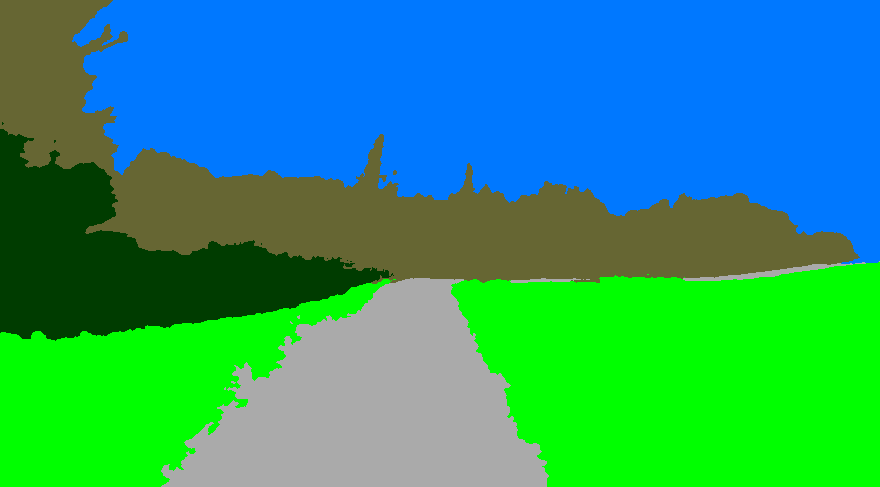
\includegraphics[width=8cm]{images/seg-map-eg}
  \end{center}
  \caption{语义分割图示例}
  \label{fig:segmentation-map-example}
\end{figure}

\subsubsection{应用}

一旦将草图转化为逼真的图像的技术成熟到足以商用,这项技术将会非常流行,设计师们可以不再仅仅依靠他们的
想象力来想象作品完成时的样子,而是可以通过栩栩如生的画面来快速预览自己的设计。例如,游戏设计师仅绘制几组色块或轮廓草图
就可以生动地预览他设想中的场景、物品、角色的样子。除此之外,这项技术还可以为不擅长美术或艺术设计的人提供了
创造出属于他们自己的艺术、设计杰作的机会。

\subsection{深度学习}

深度学习基于人工神经网络和表征学习(即自动从原始数据中发掘进行特征检测或分类所需要的表示信息\cite{wikipedia}),
是机器学习算法大家族当中的一员。深度学习可以分为监督学习、半监督学习和无监督学习。深度学习算法现已广泛应用于包括
计算机视觉(CV)、自然语言处理(NLP)、强化学习(RL)、文本过滤、机器翻译、图像合成、药物设计等在内的众多领域,
深度神经网络在这些领域的相关问题能够表现得和人类专家的水平相当,有时甚至可以做的比人类专家更好。

\subsubsection{神经网络}

人工神经网络(ANN)是一种非严格地受到构成动物大脑的神经网络启发从而发明的计算系统\cite{wikipedia}。深度学习中
所使用的神经网络可以大概视为将带有参数$\omega$的一个试图把输入A映射到输出B的逼近真实映射的函数,
即:$f_{\boldsymbol{\omega}}: A \rightarrow B$。该网络使用原始数据和反向传播算法不断更新参数,神经网络的
多层架构通过将多个非线性但简单的函数组合在一起从而实现复杂的函数映射。在实际使用的过程中,输入“信号”将通过将节点
连接的边进入节点(或称神经元),每个“信号”的输出神经元是通过其输入总和的某些非线性的激活函数来计算的。一般来说,
神经元叠加在一起形成“层”,“信号”从第一个输入层传播到最后一个输出层产生最终的结果。

\subsubsection{激活函数}

在神经网络中,一个节点(或神经元)的激活函数决定了最后输出的结果。值得注意的是,只有非线性的激活函数才能使得这些
神经网络计算出复杂的映射函数,如果我们不使用激活函数或只使用线性的激活函数,无论我们叠加多少中间层,我们最终都只能
得到线性的映射函数。下文介绍的内容引用了CS231N课件的内容\cite{cs231n}。

本项目中所用到的激活函数包括以下几种:
\begin{itemize}
  \item 线性整流函数(ReLU)
  
  线性整流函数是近几年来最简单,最常用的激活函数之一,它会计算$f(x)=\max(0,x)$这个函数。
  这个函数所做的仅仅是在零出设置阈值,相比双曲正切(tanh)或S型(sigmoid)函数要简单的多,然而,研究者发现它相比
  其它的方法(如双曲正切或S型函数)可以更快地完成梯度下降算法的收敛。不过,它也有较为脆弱这一缺点,在训练的过程中,
  线性整流单元可能因为偏离正常的数据流形从而不可逆地“死亡”并永远输出零值。 
  \begin{figure}[H]
      \begin{center}
      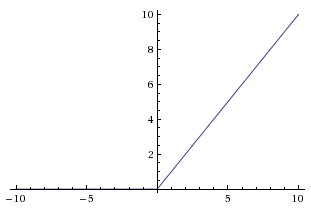
\includegraphics[width=5cm]{images/relu}
      \end{center}
      \caption{线性整流激活函数(ReLU)}
      \label{fig:ReLU}
  \end{figure}

  \item 带泄漏的线性整流激活函数(Leaky ReLU)
  
  带泄漏的线性整流激活函数是试图解决线性整流单元“死亡”的一种方法,函数不再只是设置零阈值,而是计算
  $f(x)=1(x<0)(\alpha x)+1(x>=0)(x)$这个函数,其中,$\alpha$ 是一个很小的常数。一些研究表明
  带泄漏的线性整流激活函数十分有效但是各路研究者得出的结论并不一致。
  \begin{figure}[H]
      \begin{center}
      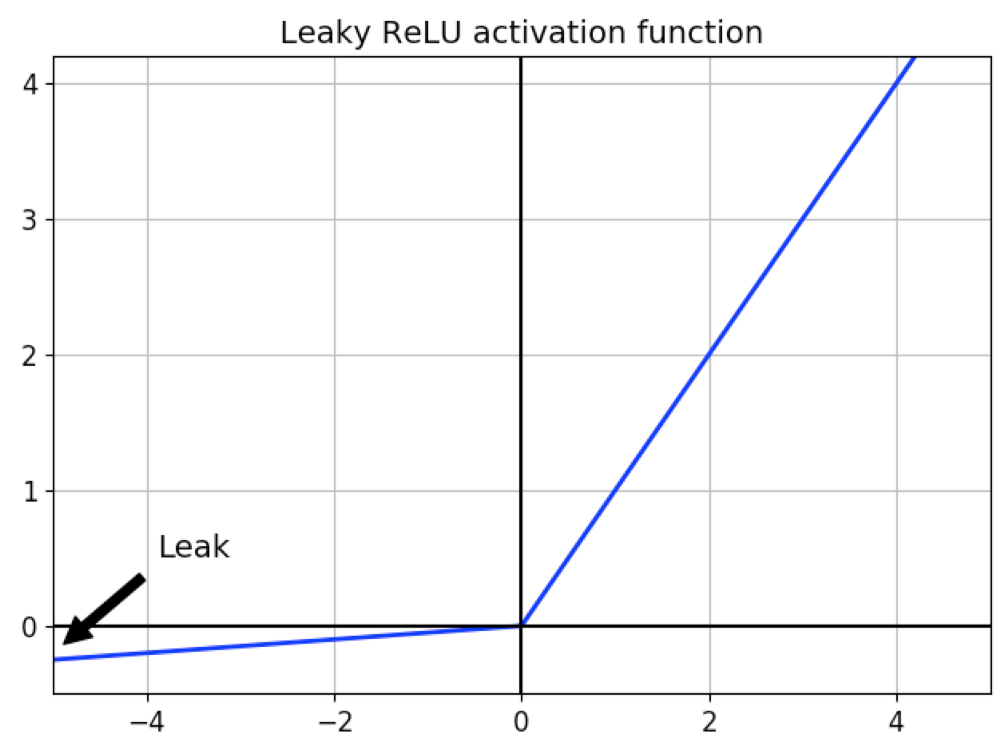
\includegraphics[width=5cm]{images/leakyrelu}
      \end{center}
      \caption{带泄漏的线性整流函数(Leaky ReLU)}
      \label{fig:Leaky ReLU}
  \end{figure}

  \item 双曲正切激活函数(tanh)
  
  双曲正切激活函数将实数的输入压缩到[-1, 1]的范围内,此激活函数饱和但以零为中心,因此可以将其视为一个由S型函数缩放
  得到,类似S型函数但是又比S型更理想的激活函数。
  \begin{figure}[H]
      \begin{center}
      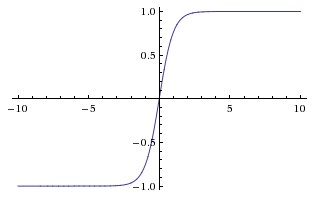
\includegraphics[width=5cm]{images/tanh}
      \end{center}
      \caption{双曲正切激活函数(Hyperbolic Tanh)}
      \label{fig:tanh}
  \end{figure}
\end{itemize}

\subsubsection{反向传播算法}

反向传播(BP)是一种广泛实用的用于神经网络训练,特别是监督学习训练的参数优化算法。在训练神经网络时,会有一个损失函数
(有时也成为目标函数)$L$,通过计算模型近似函数的输出和训练数据集中的真实值之间的差值来描述当前的近似函数
$f_{\boldsymbol{\omega}}$在多大程度上成功逼近了正确的映射函数。然后,反向传播算法就会通过不断地尝试减小损失函数
来使得模型近似函数更加贴近正确的映射函数。反向传播算法首先会利用链式法则和每对输入输出数据计算出损失函数的对于每个参数
的梯度,这个梯度计算的过程将会从最后一层开始逐渐传播到前面,每次计算一层的梯度,这样可以避免不必要的计算,每次计算梯度
之后,模型都会通过
$\boldsymbol{\omega}_{i} \leftarrow \boldsymbol{\omega}_{i}-\alpha \frac{\partial L}{\partial \boldsymbol{\omega}_{i}}$
更新一次参数${\boldsymbol{\omega}_{i}}$,其中,$\alpha(>0)$代表学习速率,$\frac{\partial L}{\partial \boldsymbol{\omega}_{i}}$
代表偏导数(即梯度)。理论上讲,梯度的方向是远离最小值的方向,所以,我们每次更新参数都是在向着模型更加贴近真实的映射函数
前进了一小步,这种优化损失函数的方法被称为梯度下降法。

\subsubsection{卷积神经网络}

卷积神经网络(CNN)是一种常被用于计算机视觉相关问题的非常流行的深度神经网络结构。典型的卷积模块由卷积层、池化层、全连接层组成。
一个简单的流程可以是:[输入-卷积-激活-池化-全连接],下面是具体说明(下文内容引用了CS231N课件\cite{cs231n}):
\begin{itemize}
  \item 输入:输入[宽, 高, 通道数]这一形式的张量将承载这输入图片的原始像素值,例如,在MNIST数据集中,每张图片的张量形式为[28, 28, 1],
  即$28\times28$分辨率且只有一个通道来表示黑白的图片。
  \item 卷积:卷积是整个卷积神经网络的关键,卷积层将计算每个连接到输入局部区域的神经元的输出,每个神经元都计算一个他们权重参数和连接到输入的小区域
  的点乘乘积。输出的张量将是[宽,高,过滤器数量]的形式,其中,过滤器的数量是一个CNN层的超参数。通过恰当的参数优化,卷积层能够从原始图片中提取
  相关的特征图,例如边缘、角落等,这将对后续的诸如图像分类、图像合成等非常有帮助。
  \item 激活:激活理解起来相对简单。一个简单的解决方案就是使用ReLU,激活函数不会影响输出的张量形状。
  \item 池化: 在大多数情况下,我们都会使用最大池化,最大池化简单来说就是一种下采样的压缩方式,减小模型的计算量,池化操作将会使输出的张量
  形状变为[宽/n, 高/n, 过滤器数量]。
  \item 全连接:全连接层,即这一层中的每个神经元都和前面一层所有神经元相连接,举个分类任务的例子,一个全连接层将计算出每个类别的得分,之后
  以[1, 1, 类别数]的形式输出,其中,每个类别都将获得一个评分用来表示某个图片有多大的概率属于这个类别。
\end{itemize}

通过这种方式,卷积神经网络将能够使原始图像从像素值转化为分类各类别的评分或编码的特征图。值得注意的是,在此项目中,我们还使用了CNN的转置,其
本质是一个CNN的逆过程,可以将特征图解码得到照片般的图像。所以,在我们的图像翻译问题中,我们一个很容易想到的解决方案就是先使用CNN将语义分割图
提取为特征图,再使用一个转置CNN模块将特征图解码为具有照片般真实感的图像。
\begin{figure}[H]
  \begin{center}
  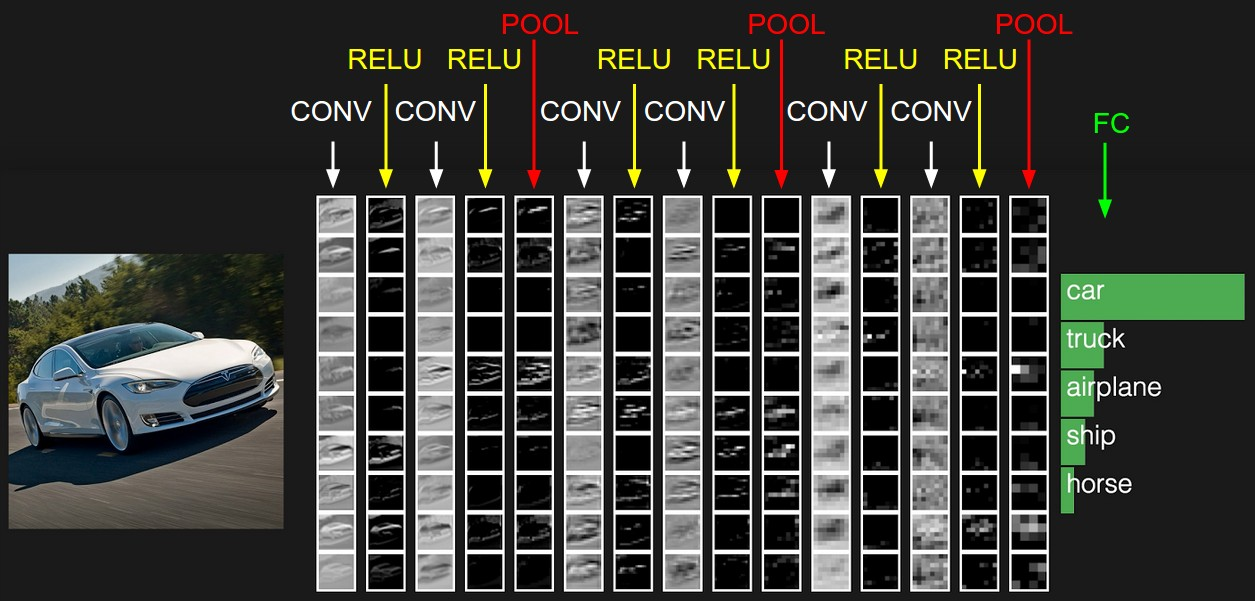
\includegraphics[width=8cm]{images/convnet}
  \end{center}
  \caption{卷积神经网络应用(分类)示例}
  \label{fig:CNN}
\end{figure}

\subsubsection{残差网络模块}

一个传统的深度学习观点是,使用更深的神经网络不一定可以得到更好的结果,实际上,研究者们发现简单地叠加大量CNN模块会由于梯度很容易缩小到零的缘故
而产生负面影响。但是,He等人\cite{he2015deep}提出的带有残差模块的残差神经网络彻底消除了这一问题。残差模块使用跳过连接的方式,将先前一层的
输出$x$添加到当前层堆叠卷积层的输出$F(x)$中,如此一来,即使在堆叠的较深的层中发生了某些错误(如梯度降至零),网络的整体还可以使用先前的未
叠加卷积层的输出。因此,残差网络可以保证我们最终得到的结果不会比浅层的网络差,最坏的情况也是和浅层网络结果相当。有了残差模块之后,
使用更深的卷积神经网络便有了在计算机视觉相关的问题中取得更好的成果的可能。
\begin{figure}[H]
  \begin{center}
  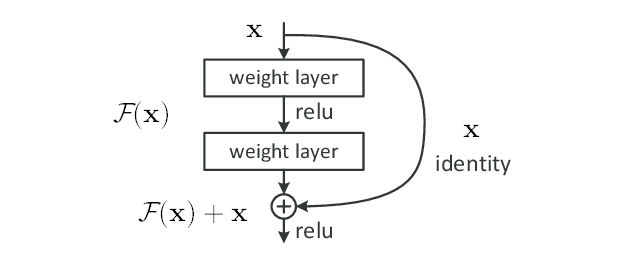
\includegraphics[width=8cm]{images/resnet}
  \end{center}
  \caption{残差网络模块的结构}
  \label{fig:Res-structure}
\end{figure}

\subsubsection{批标准化}
\label{sec:BN}
根据CS231N\cite{cs231n}的课件,批标准化处理(BN)是由Ioffe和Szegedy首次提出的,一种通过强制整个网络的激活层呈现单位高斯分布的方式来减少
神经网络训练初始化参数的麻烦的最近十分流行的技术。在深度学习的训练中,后一层从前面一层得到的输入可能是高方差和平均值和零差得很远的,这将不利于
模型稳定的训练,为了解决这个问题,批标准化对所有的数据按照如下公式进行处理:
$$y_{i}=\gamma \hat{x}_{i}+\beta \text { 以及 } \hat{x}_{i}=\frac{x_{i}-\mu}{\sqrt{\sigma^{2}+\epsilon}}$$

其中,$x_{i}$是这一批数据中的第$i$个数据,$\hat{x}_{i}$是处理后的输出,$\mu$和$\sigma^{2}$分别是这一批数据中的平均值和方差 
而$\gamma$和$\beta$是可训练的参数。

在实际应用过程中,我们通常在全连接层和非线性层之间插入批标准化处理,研究者们实验发现使用批标准化处理可以使得神经网络对不佳的初始化拥有更好的稳定
性和容错率。此外,批标准化处理可以当作是集成在网络当中的,在网络的每层进行的预处理,非常容易实现,这就是为什么批标准化处理如今使用如此广泛的原因。
如需了解关于批标准化的更多内容请参考Ioffe的论文\cite{ioffe2015batch}。

\subsection{生成对抗网络}

生成对抗网络(GAN)是一种由Goodfellow等人提出的深度学习方法\cite{Goodfellow-et-al-2016}。生成对抗网络的思路受到博弈论的启发:两个神经网络
在深度学习的训练过程中相互竞争,一个是生成器网络试图生成以假乱真的逼真假图,而另一个是辨别器网络目标是识别某张图片是真实的还是生成器伪造的。生成
对抗网络的损失函数可以是对输出图像的分类准确度,然后通过不断地尝试最小化损失函数来训练生成器。在图像翻译的问题上,生成对抗网络的一个很明显的优势
就在于其可以生成更加清晰的图像,因为模糊的图像显然是伪造的。此外,我们也并不需要像设计传统卷积神经网络那样针对特定的任务来设计十分复杂的损失函数,
在这里我们只需要给生成对抗网络一个简单的宏观目标:“让伪造的输出看起来像是真的”即可。然后训练中生成器会和辨别器互相博弈,从而实现这个目标。
\begin{figure}[H]
  \begin{center}
  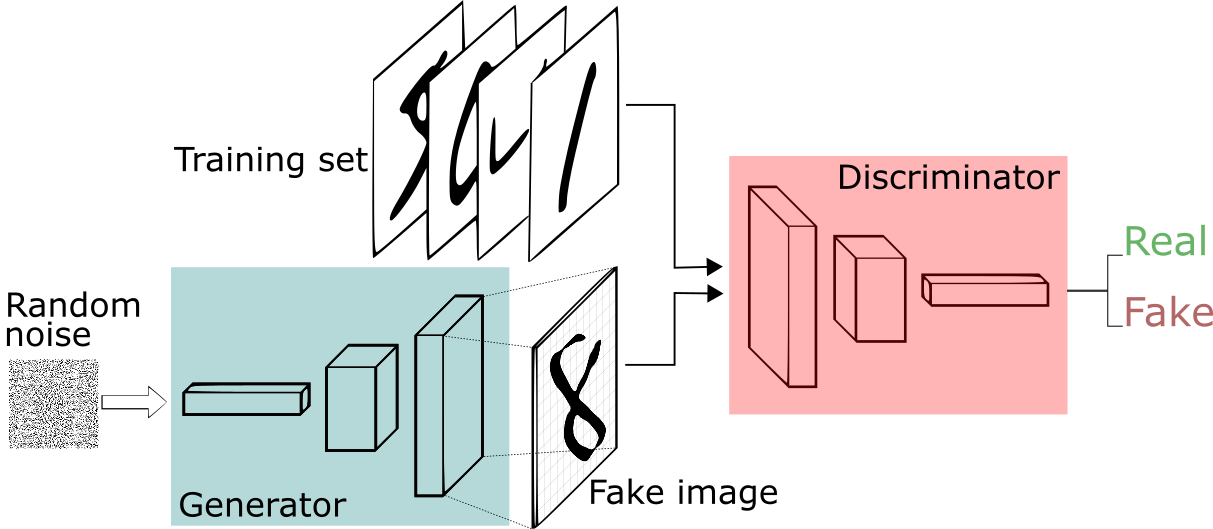
\includegraphics[width=8cm]{images/GANs}
  \end{center}
  \caption{生成对抗网络的结构}
  \label{fig:GANs-structure}
\end{figure}

\subsubsection{条件生成对抗网络}

条件生成对抗网络(cGAN),是一种特殊的生成对抗网络,其输入不再只是像普通生成对抗网络一样的随机噪声,而且还会附带条件的数据。神经网络将会学习并调整
参数来适应这些附加的输入条件。在传统的生成对抗网络模型中,对输入而言只有噪声会影响最后的输出,但是对于条件生成对抗网络而言,条件也会影响输出。
条件生成对抗网络是最先在图像翻译的任务中使用的方法,而语义分割图就是我们给生成对抗网络的条件。著名的模型Pix2pix\cite{pix2pix2016}
和Pix2pixHD\cite{wang2018pix2pixHD}就是对条件生成对抗网络的应用。

\begin{figure}[H]
  \begin{center}
  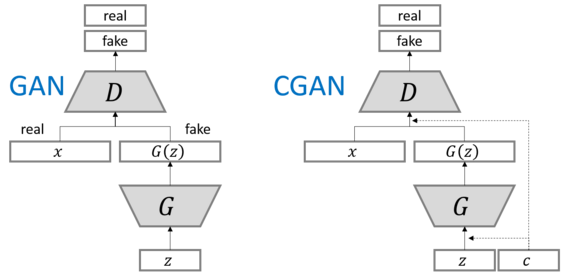
\includegraphics[width=10cm]{images/cGANs}
  \end{center}
  \caption{条件生成对抗网络结构}
  \label{fig:cGANs-structure}
\end{figure}

\section{文献综述}

本章节将会通过介绍三个具有代表性的模型来探讨用生成对抗网络方式解决图像翻译问题的起源和发展,对于后两个最前沿的模型Pix2pixHD和SPADE,本章节只讲述原理,
具体的实现细节和实验测试将在第\ref{sec:four}章讨论。

\subsection{基于条件生成对抗网络的图像翻译}

使用生成对抗网络来解决图像翻译问题由Isola等人最先提出。他们尝试使用条件生成对抗网络的原理开发一个通用的架构来处理全部的
“由像素预测像素”的问题。他们的这项研究可以在较简单的数据集的训练下生成$256\times256$分辨率的图像。后文的内容参考了他们的论文\cite{pix2pix2016}。

\subsubsection{损失函数}

模型的目标是根据给定的语义分割图,伪造出足以以假乱真的图片,整个条件生成对抗网络的损失函数为:
$$\mathcal{L}_{c G A N}(G, D)=\mathbb{E}_{x, y}[\log D(x, y)]+\mathbb{E}_{x, z}[\log (1-D(x, G(x, z))]$$
其中,生成器$G$试图最小化损失函数但是辨别器$D$却与之对抗试图最大化损失,即$G^{*}=\arg \min _{G} \max _{D} \mathcal{L}_{c G A N}(G, D)$。
在代码实现的阶段,生成对抗网络的损失通常由真损失和假损失两部分组成,真假损失代表了辨别器对于识别真图片和假图片的能力,生成器的目标就是最大化辨别器
输出的对于它所伪造的图片为真的概率。

论文中还强调将生成对抗损失和我们常用的损失例如$L1$损失结合效果会更好:$\mathcal{L}_{L 1}(G)=\mathbb{E}_{x, y, z}\left[\|y-G(x, z)\|_{1}\right]$。
那么现在我们的整个模型的损失函数就是:
$$G^{*}=\arg \min _{G} \max _{D} \mathcal{L}_{c G A N}(G, D)+\lambda \mathcal{L}_{L 1}(G)$$

值得注意的是,我们在Pix2pix模型中,并不需要提供噪声输入,因为我们只需要确定的输出即可,而随机噪声对于最终结果并不会有很大的帮助。
\begin{figure}[H]
  \begin{center}
  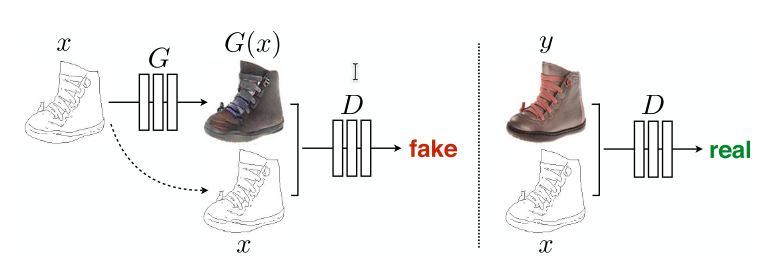
\includegraphics[width=10cm]{images/pix2pix-cGAN}
  \end{center}
  \caption{Pix2pix模型中的条件生成对抗网络}
  \label{fig:pix2pix-cGAN}
\end{figure}

\subsubsection{模型结构}

生成器和辨别器均使用了[卷积-批标准化-激活]这样的卷积模块,生成器使用了经典的编码-解码结构,其中,编码器负责从语义分割图中提取
特征图,解码器负责填充图片的细节并结合特征图生成如照片般逼真的图像。另外,对于图像翻译的任务来说,编码层与解码层分享一些信息将
对任务十分有帮助,所以,作者使用了一种“U”型网络的连接方式将第$i$层与对应的$n-i$层连接起来,其中$n$是总层数,连接的方式就是简单的
将所有通道拼接起来。对于辨别器而言,作者使用了PatchGAN的结构,具体来说就是将整个图像分割成一个个$N \times N$的小块,然后让辨别器
分辨每个小块是真是假,这样的好处就是使用更少的参数,更快的运行速度以及处理更体积更大图片的潜力。
\begin{figure}[H]
  \begin{center}
  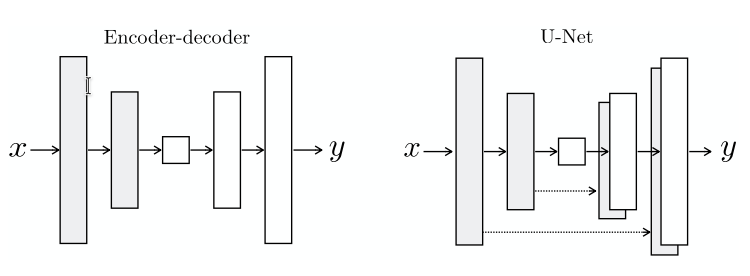
\includegraphics[width=12cm]{images/pix2pix-generator}
  \end{center}
  \caption{编码-解码结构生成器 VS. “U”型网络结构生成器}
  \label{fig:pix2pix-generator}
\end{figure}

\subsubsection{总结}

Pix2pix模型不需要很多的计算资源,我们甚至可以直接在谷歌Colab平台上进行训练,我尝试着按照谷歌Tensorflow官方的教程\cite{tf-pix2pix-tutorial}
跑了这个模型的训练,下图就是其在facade数据集\cite{Tylecek13}上训练了100个周期(epoch)后的结果:
\begin{figure}[H]
  \begin{center}
  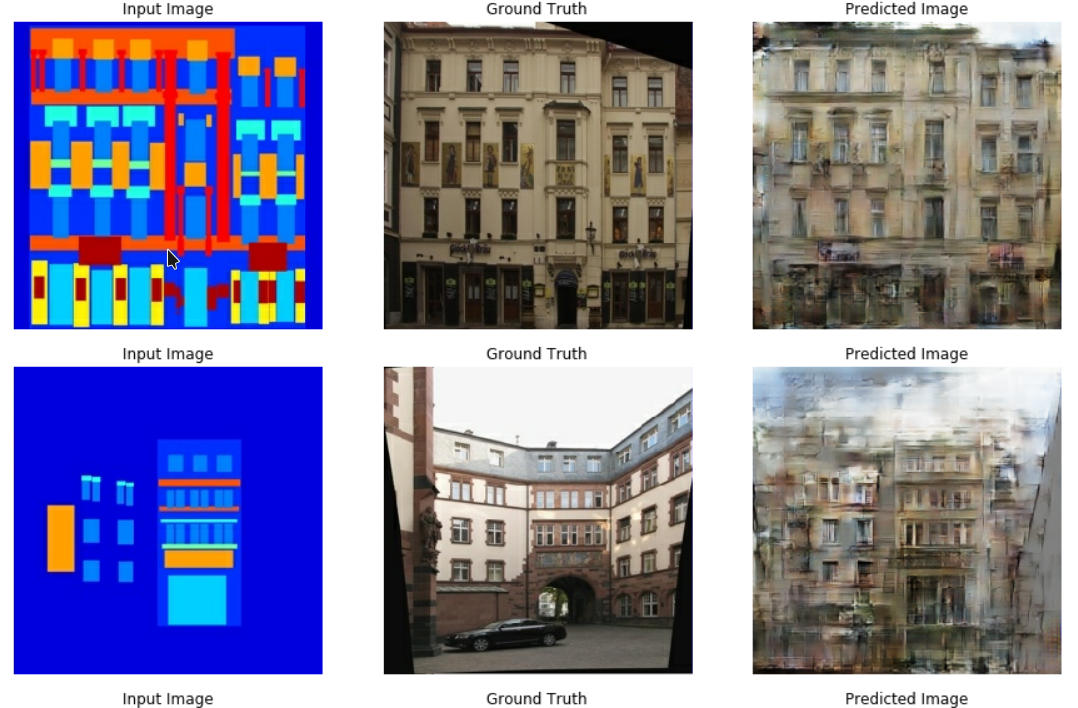
\includegraphics[width=12cm]{images/pix2pix-output}
  \end{center}
  \caption{Pix2pix模型的输出图像示例}
  \label{fig:pix2pix-output}
\end{figure}

根据我自己以及论文中的实验结果来看,我发现Pix2pix模型即使只用有限的算力和较简单的数据集也是能够生成比较清晰的图像的。然而,它依然存在着不足,比如
对于某些区域无法生成清晰的纹理,以及无法生成高分辨率的图像。

\subsection{当前最先进模型之一 —— Pix2pixHD模型}

Pix2pixHD模型是由英伟达提出的Pix2pix模型的升级版,它旨在解决高分辨率图像的生成问题。在论文\cite{wang2018pix2pixHD}中,作者们成功借助Cityscapes
数据集\cite{Cordts2016Cityscapes}生成了分辨率高达$2048\times1024$的图像。Pix2pixHD模型依然是基于条件生成对抗网络实现的,但是它对Pix2pix的
生成器、辨别器、损失函数均做出了改进。后文参考了原论文\cite{wang2018pix2pixHD}的内容。

\subsubsection{生成器}

生成器$G$由两个子生成器组成,我们定义$G1$为全局生成器,$G2$为局部强化器,全局生成器的作用和Pix2pix模型相似,基本上是一个编码器-解码器的结构并采用了
残差网络模块用来输出低分辨率的图像,然后再使用局部强化器将低分辨率的图像进一步提升为高分辨率的图像。无论是全局生成器还是局部强化器都是由卷积网络模块、
残差网络模块、转置卷积网络模块组成的,我们分别用$G_{1}^{(c)}$, $G_{1}^{(r)}$, $G_{1}^{(t)}$以及$G_{2}^{(c)}$, $G_{2}^{(r)}$, 
$G_{2}^{(t)}$来命名。为了将这两个生成器整合到一起,输入到局部强化器的残差网络模块的输入是$G_{2}^{(c)}$的特征图和$G_{1}^{(t)}$最后的特征图按元素
求和的结果。整个生成器的结构图如下:
\begin{figure}[H]
  \begin{center}
  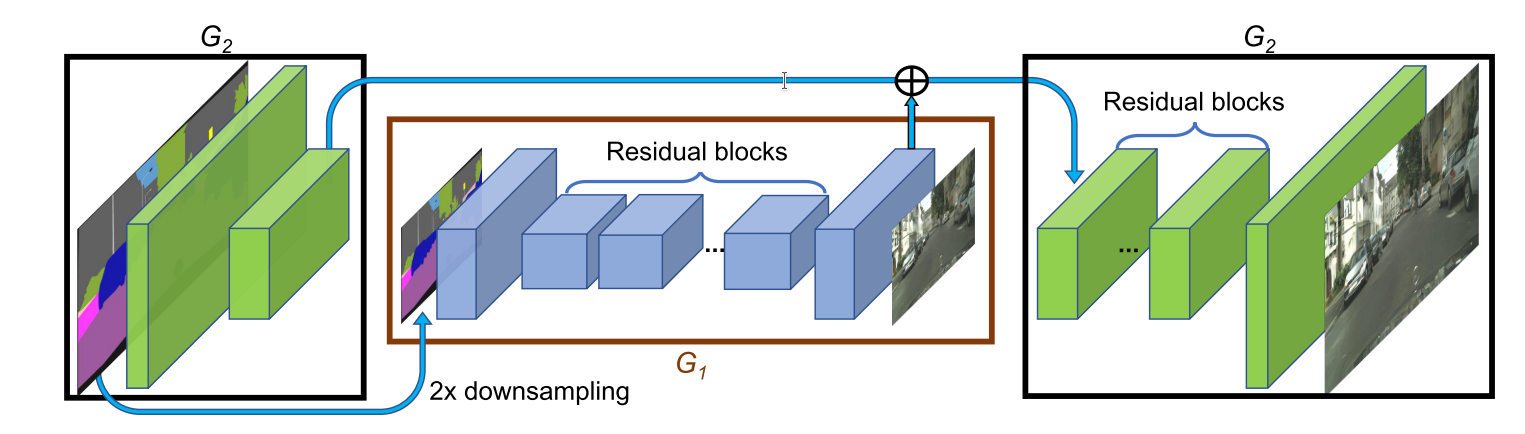
\includegraphics[width=12cm]{images/pix2pixHD-generator}
  \end{center}
  \caption{Pix2pixHD生成器结构}
  \label{fig:pix2pixHD-generator}
\end{figure}

训练生成器的过程中,我们需要先训练好全局生成器,然后再去训练局部强化器和微调。

\subsubsection{辨别器}

辨别器$D$在Pix2pixHD模型中被升级成了多重缩放辨别器,减少了为提高感知面积所需要的算力提升的麻烦,毕竟算力永远都是稀缺资源。所以,多重缩放辨别器所做的
就是使用三个小辨别器分别作用于三种不同程度缩放后的图像,例如,作者使用了$D1$, $D2$, $D3$三个结构相同的辨别器分别作用于2倍、4倍缩放的图像以及原图,
作用于精细缩放图像的辨别器重点辨别图像的细节,同时作用于粗略缩放图像的辨别器重点放在了大局观的感知上。在代码实现的时候,我们只需要累加三个辨别器的损失
函数即可将它们的效果综合起来,最终的生成对抗网络的minimax表达式变为:
$$\min _{G} \max _{D_{1}, D_{2}, D_{3}} \sum_{i=1,2,3} \mathcal{L}_{\mathrm{GAN}}\left(G, D_{i}\right)$$

\subsubsection{损失函数}

改进后的损失函数由以下几个部分组成:
\begin{itemize}
  \item 生成对抗网络损失:和之前Pix2pix模型的相似: 
  $$\mathcal{L}_{G A N}(G, D)=\mathbb{E}_{x, y}[\log D(x, y)]+\mathbb{E}_{x}[\log (1-D(x, G(x))]$$
  \item 特征图损失:一个辨别真伪的想法是匹配真假图片的中间过程的卷积结果,所以在Pix2pixHD模型中我们提取了辨别器中每一层的特征图,并计算得到
  每一层的特征图损失,然后在把所有的特征图损失加起来:
  $$\mathcal{L}_{\mathrm{FM}}\left(G, D_{k}\right)=\mathbb{E}_{(\mathbf{s}, \mathbf{x})} \sum_{i=1}^{T} \frac{1}{N_{i}}\left[\left\|D_{k}^{(i)}(\mathbf{s}, \mathbf{x})-D_{k}^{(i)}(\mathbf{s}, G(\mathbf{s}))\right\|_{1}\right]$$
  
  其中,$D_{k}^{(i)}$是辨别器$D_{k}$第$i$层的特征提取器, $T$是总层数,$N_{i}$是每层元素的数量。
  \item (可选)VGG损失:VGG损失也称为感知损失,我们可以借助预训练好的VGG网络的模型\cite{articleVGG}来计算此损失: 
  $\lambda \sum_{i=1}^{N} \frac{1}{M_{i}}\left[\left\|F^{(i)}(\mathbf{x})-F^{(i)}(G(\mathbf{s}))\right\|_{1}\right]$,
  
  其中,我们选择让$\lambda=10$,$F_{i}$是第$i$层的映射函数,其中包含了$M_{i}$个VGG网络的元素。
\end{itemize}
最终不包含VGG损失的损失函数为:
$$\min _{G}\left(\left(\max _{D_{1}, D_{2}, D_{3}} \sum_{k=1,2,3} \mathcal{L}_{\mathrm{GAN}}\left(G, D_{k}\right)\right)+\lambda\sum_{k=1,2,3} \mathcal{L}_{\mathrm{FM}}\left(G, D_{k}\right)\right)$$
包含了VGG损失的损失函数为:
$$\min _{G}\left(\left(\max _{D_{1}, D_{2}, D_{3}} \sum_{k=1,2,3} \mathcal{L}_{\mathrm{GAN}}\left(G, D_{k}\right)\right)+\lambda\sum_{k=1,2,3} \mathcal{L}_{\mathrm{FM}}\left(G, D_{k}\right) + \lambda \sum_{i=1}^{N} \frac{1}{M_{i}}\left[\left\|F^{(i)}(\mathbf{x})-F^{(i)}(G(\mathbf{s}))\right\|_{1}\right]\right)$$

\subsection{当前最先进模型之一 —— SPADE模型}

SPADE全称空间适应性标准化,是英伟达提出的又一种对图像翻译问题的改进方案。之前我们讲到的Pix2pix和Pix2pixHD模型都是基于条件生成对抗网络这一结构的,
使用这种结构,我们都会将语义分割图直接当作输入给到生成器,使语义分割图经过一系列的卷积、残差、非线性激活等层的处理。SPADE论文\cite{park2019SPADE}
作者发现在标准化的过程中许多图片的细节将会被抹除,因此,作者提出了一种不再是依靠两个可训练参数,而是结合了语义分割图信息的新型标准化层。SPADE模型直接
采用了Pix2pixHD模型对于辨别器和损失函数的设计,所以下面我们将主要讨论SPADE改进比较大的生成器这一部分。下文内容参考了原论文\cite{park2019SPADE}。

\subsubsection{SPADE模块}

SPADE模块是整个SPADE生成器的关键所在,与批标准化处理相似,以通道为基准标准化按如下公式处理激活函数的输出(我们在批标准化的小节\ref{sec:BN}解释过):
$$y_{i}=\gamma \hat{x}_{i}+\beta \text { 以及 } \hat{x}_{i}=\frac{x_{i}-\mu}{\sqrt{\sigma^{2}+\epsilon}}$$

然而,不同的是,在SPADE模块中,$\gamma$和$\beta$不再是可训练参数而是直接通过一个作用于输入语义分割图的两层卷积网络计算得到,由于现在标准化处理的
重要参数是直接受输入的语义分割图影响的,因此我们无需再担心语义信息被标准化过程抹去了。SPADE模块的结构示意图如下:
\begin{figure}[H]
  \begin{center}
  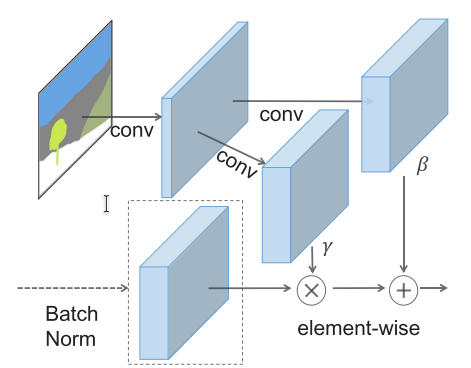
\includegraphics[width=5cm]{images/SPADE-Block}
  \end{center}
  \caption{单个SPADE模块的结构图}
  \label{fig:SPADE-Block}
\end{figure}

\subsubsection{SPADE残差模块}

SPADE残差模块是被用来替代传统的残差模块的,不再是像传统方式一样只使用卷积层,SPADE残差模块还使用了上一小节提到的SPADE模块,通过加入SPADE模块的方式,
我们成功的将输入的语义分割图的语义信息集成到了残差模块当中。整个SPADE残差模块的结构示意图如下:
\begin{figure}[H]
  \begin{center}
  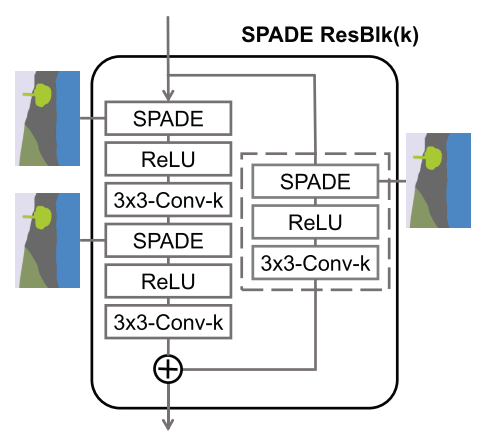
\includegraphics[width=5cm]{images/SPADE-ResBlock}
  \end{center}
  \caption{单个SPADE残差模块结构示意图}
  \label{fig:SPADE-ResBlock}
\end{figure}

\subsubsection{生成器}

距离完成完整的生成器,我们只需要做将SPADE残差模块放入生成对抗网络当中这最后一步即可。由于我们已经通过残差模块读入了语义分割图的语义信息,所以我们不再像之前
一样需要条件生成对抗网络的编码器来输入语义分割图,我们可以使用普通生成对抗网络的结构,使用随机噪声当作输入即可。所以现在SPADE生成器的结构如下图:
\begin{figure}[H]
  \begin{center}
  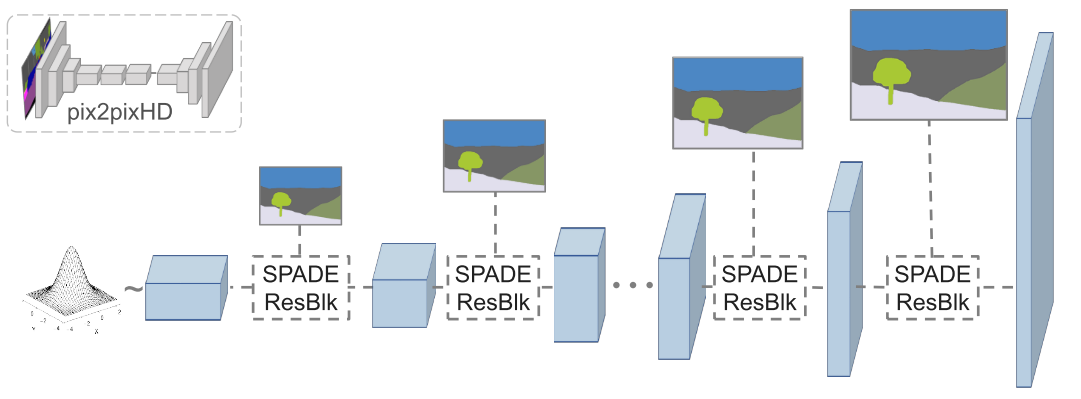
\includegraphics[width=12cm]{images/SPADE-generator}
  \end{center}
  \caption{SPADE生成器结构示意图}
  \label{fig:SPADE-generator}
\end{figure}

\subsubsection{变分自动编码器}

除了对生成器的改进之外,SPADE还对生成对抗网络损失改为了Hinge损失,使用了谱标准化等小改进。此外,由于不再需要编码器读入输入图像,我们可以使用一个
变分自动编码器来实现风格迁移的效果,加入了变分自动编码器的完整SPADE模型框架图如下:
\begin{figure}[H]
  \begin{center}
  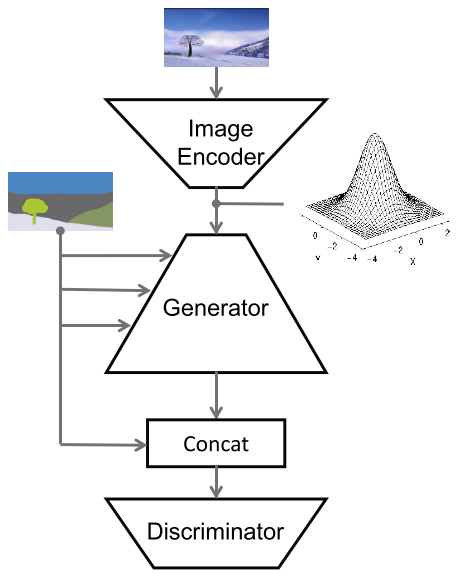
\includegraphics[width=5cm]{images/SPADE-architecture}
  \end{center}
  \caption{SPADE生成对抗网络结构示意图}
  \label{fig:SPADE-architecture}
\end{figure}

变分自动编码器将编码一张风格图片,产生用于后续计算提供给生成器噪音的一个平均值和一个方差值。辨别器会读入语义分割图和生成器输出的图像拼接而成的图像
来判断图片是真还是假。

\section{项目开发综述}

本文在这个章节将会介绍项目开发的相关内容,诸如使用到的开发工具,深度学习训练使用的计算平台,图形界面开发等。

这个项目尝试着实现Pix2pixHD和SPADE两个前沿的图像翻译模型并且尝试让他们不但能处理数据集的图像,也可以根据自由绘制的分割图来生成图片。因此,整个
项目分为两个部分,一个是训练深度神经网络的模型,另一个是开发一个可以展示模型能力的带有图形界面的应用。由于训练深度神经网络需要使用到我笔记本没有的GPU
算力,所以我的计划是在提供了免费GPU使用的谷歌Colab平台中训练模型,然后下载模型到本地,放入本地开发的图形界面应用中使用。

\subsection{计算资源}

谷歌推出的Colaboratory服务,通常被称为谷歌Colab,是一个以jupyter notebook的形式呈现的免费的Python在线交互环境。我们可以像在本地使用jupyter 
notebook那样在上面编写或运行Python代码,Colab已经预装了大部分供数据科学和机器学习使用的库,同时它还提供一块免费的GPU(每次会话随机分配K80,T4, 
P4,P100之一)。不过,它也并非完美,比如说,为了避免长时间占用资源我们会经常被切断与服务器的连接,而且如果长时间使用GPU训练模型的话还可能被封号
一两天。借助Colab允许我们挂载谷歌网盘的特点,我的解决方案就是将训练过一定量周期的模型数据保存在谷歌网盘中,这样即便是遇到断开连接的情况,之前训练的
结果也不会丢失,还可以继续训练。即使有诸多不便,但是这是我能想到的最好的方案了。

\subsection{深度学习框架}

这个项目所使用的深度学习框架是来自脸书公司的开源框架Pytorch。Pytorch是著名深度学习框架Torch的Python版本,为我们提供了能够使用GPU加速的张量计算,
以及基于自动求导机制的神经网络快速搭建工具,近年来在学术界正越来越流行。从一方面讲,Pytorch对于新手来说十分友好,因为我们可以很容易理解每一行代码是
在做什么,同时,Pytorch为我们定义好了诸如卷积模块、批标准化模块在内的许多常用的神经网路组件,所以十分利于快速构建原型。另一方面,它也支持研究者们用
它来搭建具有复杂结构的神经网络,这点上Pytorch要比Keras等著名的框架更有优势。最著名的深度学习框架Tensorflow使用静态图的方式构建网络,而Pytorch则
与之不同地采用了动态图的方式,这样更有助于微调和排出故障。而最让我认为Pytorch强于Tensorflow的地方在于Pytorch的文档更加清晰易读。比如说,你可能会
在Tensorflow的文档中看到不同的包中含有好几个具有相同功能的不同函数,而Pytorch就没有这种情况。如果想了解更多的信息,可以前往Pytorch的官网
\href{https://pytorch.org/}{https://pytorch.org/}。

\subsection{图形化界面}

对于展示应用程序的图形化界面,我决定采用网页应用的方式。不同于C++和$C\sharp$这样的语言,Python没有强大的桌面图形化界面的框架,然而,供Python开发者
网页开发的像Django或Flask框架却可以方便地和Pytorch的Python库整合,而且我们也可以使用框架中的模板系统与前端开发的技术结合构建一个不错的带图形化界面
的系统。当用户在图形化界面(即前端)执行一个操作时,前端就会向后台发送一个请求,然后我们的Flask框架就可以处理这项请求并在必要的时候让Pytorch的模型去
执行图像翻译的操作。

项目的前端部分基本上是由HTML、CSS、JavaScript以及如Bootstrap、Font Awesome这类相关库开发而成的。后端则是选择了Flask框架,Flask是一个轻量级WSGI
的Python网页开发框架,Flask的项目的前期开发十分的快速和简洁,但是我们也可以通过不断地添加组件来实现更复杂的功能,它整合了Jinja2模板引擎使开发者可以
让Flask后端与前端图形化界面整合在一起。

整个网页应用包括了4个页面:主页、关于项目页面、展示模型翻译数据集中的图像的页面、以及展示模型翻译用户自由绘制的图像的页面。
\begin{figure}[H]
  \begin{center}
  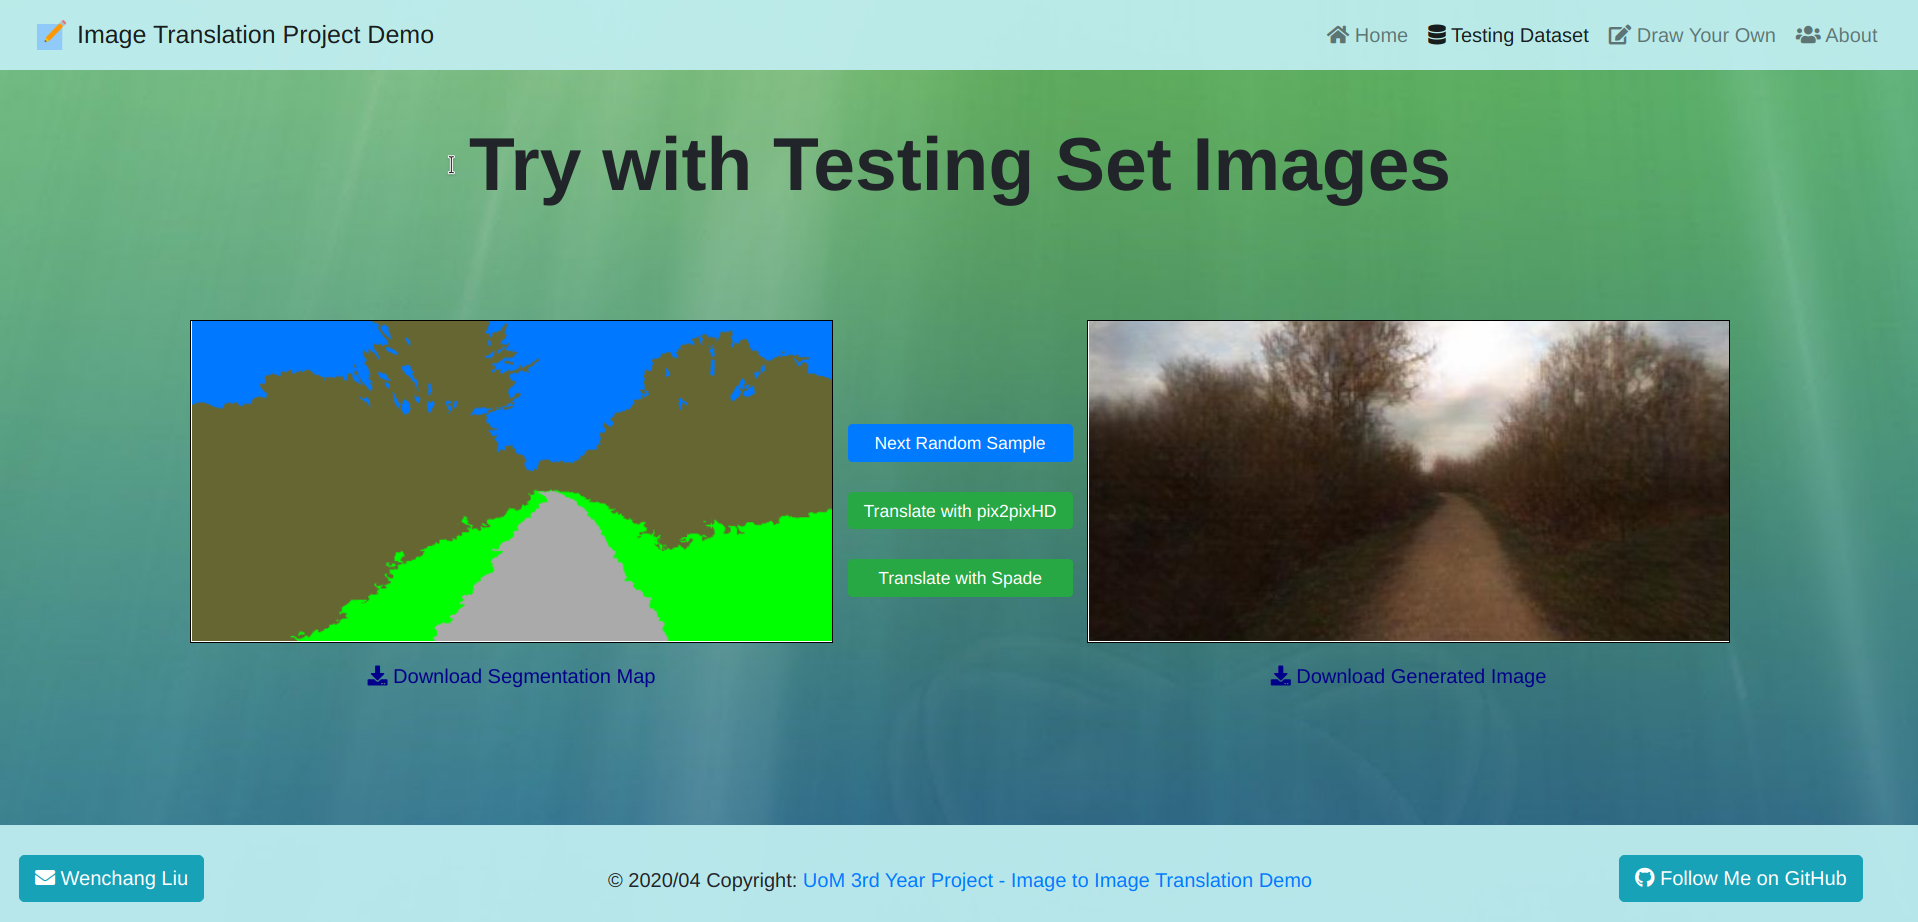
\includegraphics[width=14cm]{images/GUI-testset}
  \end{center}
  \caption{允许用户翻译数据集中语义分割图的网页截图}
  \label{fig:GUI-testset}
\end{figure}

\begin{figure}[H]
  \begin{center}
  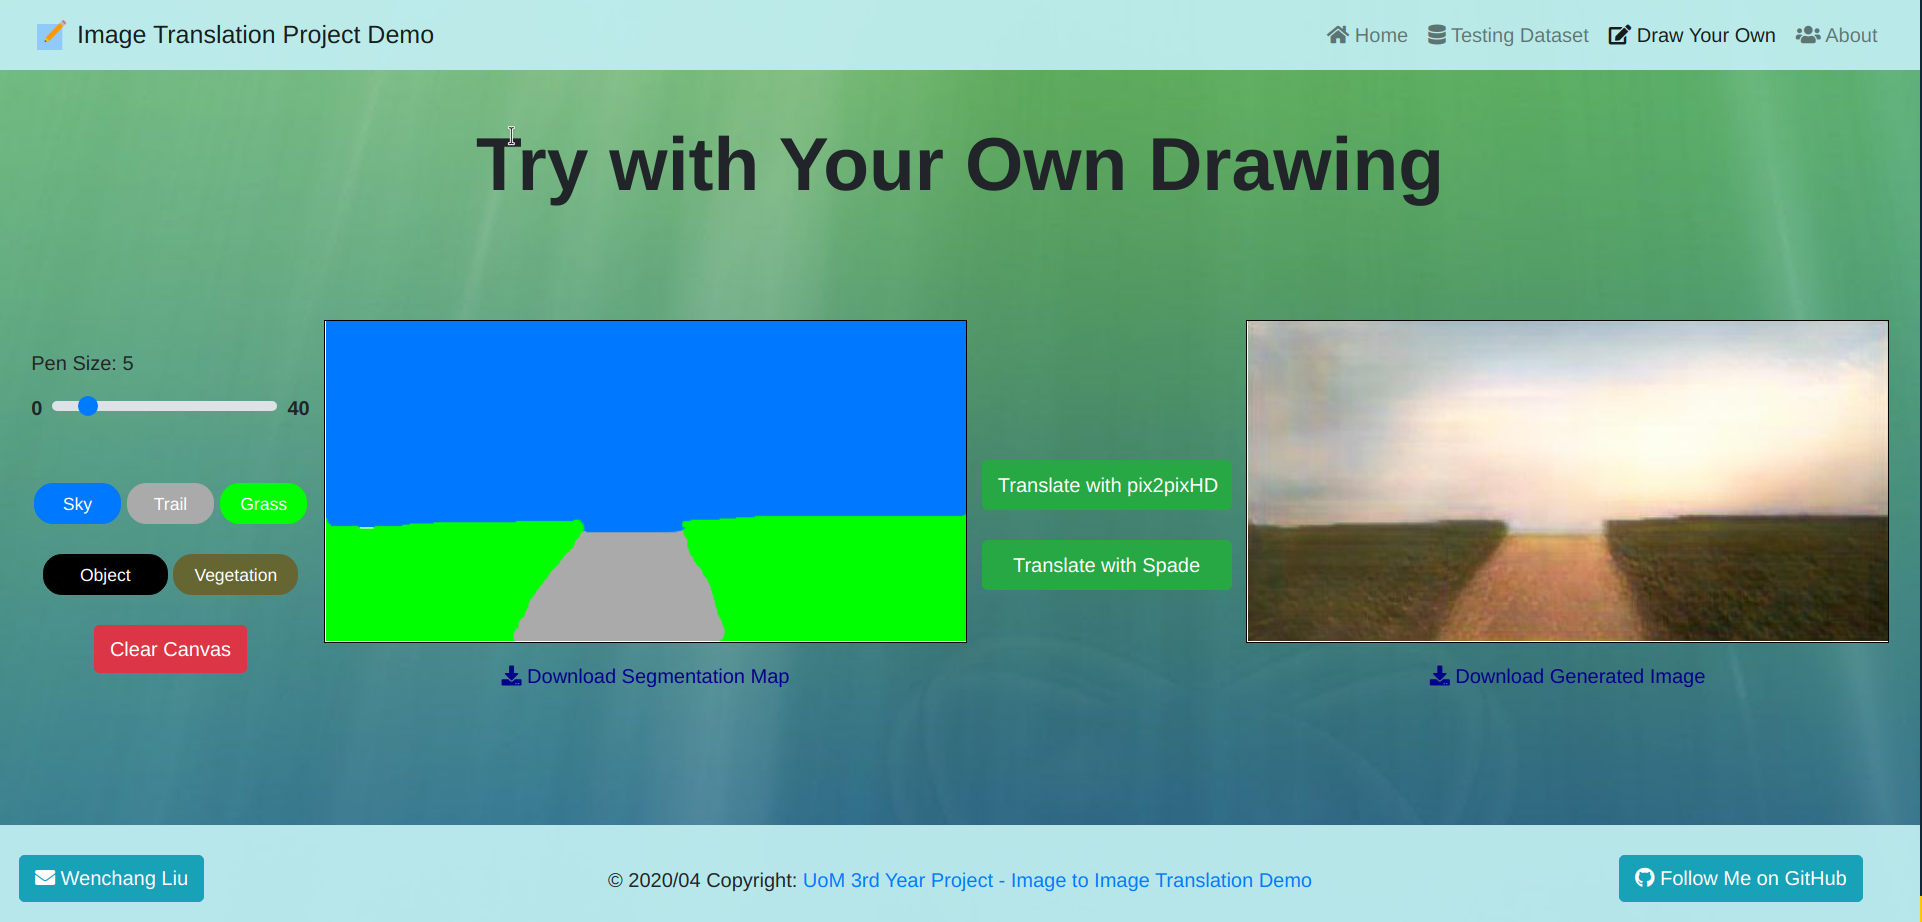
\includegraphics[width=14cm]{images/GUI-draw}
  \end{center}
  \caption{允许用户翻译自己自由绘制语义分割图的网页截图}
  \label{fig:GUI-draw}
\end{figure}

正如图\ref{fig:GUI-testset}和图\ref{fig:GUI-draw}所展示的,整个网页应用提供了读入数据集中下一个语义分割图,简单的语义分割图绘制工具,下载
语义分割图和最终生成图片,以及选择使用Pix2pixHD或SPADE模型进行图像翻译等功能。

使用方法也非常的简单,用户只需要在左侧读入或绘制语义分割图,然后按下翻译的按钮(Pix2pixHD或SPADE),之后生成的照片一样的图像就会出现在右边的窗口了。

\section{实验与评估}
\label{sec:four}

在此章节中展示了两个当前先进的模型的实现细节以及他们的测试结果和评估。由于只有Colab提供的免费GPU可用,而先进模型的训练又需要很长的时间,我决定
在我的项目中使用一个更为简单的数据集\cite{valada16iser}代替基准数据集。另外,由于SPADE的实现基于Pix2pixHD,唯一的不同就在于生成器,所以
一些在Pix2pixHD上进行的实验内容并没有在SPADE模型上重新再做。

\subsection{数据集}

训练Pix2pixHD模型的过程中,我尝试了不同的训练集,包括ADE20K\cite{zhou2017scene},Cityscapes\cite{Cordts2016Cityscapes}在内的
基准训练集,以及更为简单的Freiburg森林数据集\cite{valada16iser}。根据我的实验,我认为Freiburg森林数据集最适合此项目。

\subsubsection{基准数据集}

对于图像翻译的任务而言,我们需要的数据是成对的语义分割图和对应的照片般的图像,这样的数据和语义分割任务所需要的一样。所以,几个流行的包括
Coco-Stuff\cite{caesar2018cvpr}, ADE20K\cite{zhou2017scene}, Cityscapes\cite{Cordts2016Cityscapes}在内的基准数据集都
可以使用。我也尝试了ADE20K和Cityscapes这两个基准数据集:
\begin{itemize}
  \item ADE20K数据集\cite{zhou2017scene}是一个为了语义分割训练的人工标注的数据集,包含了20210张训练数据图像,2000张验证数据图像以及3000张
  测试数据图像。所有的标注图像都使用了不同的颜色标注了不同类别的物体,有一部分图像甚至还详细标注了物体内部的组件。与Cityscape数据集只有城市
  一种场景不同的是,ADE20K包含了机场、房屋、医院等多种场景,这使得我们的模型训练难度进一步加大,因为某些物体每次出现的时候周围的环境都可能
  不同。这个数据集大小在4GB左右。
  \item Cityscapes数据集\cite{Cordts2016Cityscapes}是一个旨在分析城市街景语义的数据集,包括了50多个城市、春夏秋三个季节、不同的天气情况、
  30个类别的物体的场景,它一共拥有5000张精细标注的图像可用。由于真实照片的分辨率较高,整个数据集大小在11GB左右,同时,物体类别过多也为模型生成
  对应的纹理增大了难度。
\end{itemize}

如果我们想要在测试集上取得不错的效果,我们就需要使用数据集中全部的训练数据,这样才能保证我们的模型能够适应测试集中的各种场景以及各种物体的纹理。
然而,就算大小最小的ADE20K数据集也有4GB大,仅有一块Colab免费GPU的情况下使用全部训练数据可能每次训练都需要几天的时间才能够完成,所以我在后面
实验的过程中,都只是用了整个训练数据集的一部分从而将训练时间控制在可以接受的范围内。

\subsubsection{Freiburg森林数据集}
\label{sec:forest}

Freiburg森林数据集\cite{valada16iser}是一个使用搭载了20HZ支持$1024\times768$分辨率的相机的无人机拍摄的照片和对应的标注好的语义分割图组成
的数据集。标注的分割图只含有5个不同的类别,分别是小路、草、天、植物以及其他物体,训练集拥有230对图片(每一对由一张照片和一张语义分割图组成),
测试集拥有126对图片,小规模的数据集增大了训练的容错率,因为我不需要等待好几个小时才能通过中间结果知道对错然后再从头再来一遍了。由于场景单一而且物体
类别也相对简单,所以我们也不需要像基准数据集那么多的训练数据了,这一点上也弥补了算力不足的缺陷。不过,即使这是一个相对较小的数据集,完整训练一个模型
仍然需要几个小时的时间才能完成。如果想要下载这个数据集或者查看更多相关信息,请访问\href{http://deepscene.cs.uni-freiburg.de}{DeepScene}的
网站。

\subsubsection{数据预处理}

Pytorch允许开发者使用“CustomDataset”方法动态地从文件夹中读入图像,所以就预处理而言,我们只需要用“glob”方法找到每一对语义分割图和对应的真实照片
所在的文件路径,然后再用PIL库将其剪裁至想要的分辨率(比如在这个项目中我们用$512\times256$的分辨率),然后将处理结果返回给Pytorch即可完成预处理。

数据增强技术也是可以用的,但是在运行Pix2pix教程的过程中我没有感觉到数据增强带给生成图片质量的明显提升,所以我在这里并没有使用数据增强的方法处理图片。

\subsection{Pix2pixHD模型实现}

本项目Pix2pixHD模型的实现基本上遵循了论文中的模型结构,只不过我减少了残差模块的数量,关于生成器的结构,可以参考图\ref{fig:pix2pix-generator}和
表\ref{Pix2pixHD generator table},辨别器的结构则可以参考表\ref{Pix2pixHD discriminator table}。最终的方案是使用Freiburg森林数据集训练,
调整分辨率至$512\times256$,并且加入在总损失函数中加入VGG损失。在得到最终方案之前,我使用一小部分的ADE20K数据集来确认VGG损失是否对结果有显著影响,
另外,我还使用Cityscapes数据集试图达到与论文中相似的结果,不过这些尝试都或多或少出现了一些不好解决的问题。

训练方面,模型使用了最常见最流行的Adam优化器。针对生成器训练难度要远大于辨别器这个特点,我为生成器设置了一个较大的学习速率而不是如论文中那样为生成器和
辨别器设置一样的学习速率,因为我发现辨别器的损失会下降的非常快,通常只需要几个周期的训练即可达到一个很低的水平,而生成器则需要大量的训练,所以我希望
这样的学习速率可以加速生成器的训练。最后生成器的学习速率为$2\times10^{-5}$,辨别器的学习速率为$10^{-5}$,效果似乎不错。

整个生成对抗网络的训练是一个循环进行的过程,在每一个周期中:
\begin{enumerate}
  \item 从训练集中取出一对图像数据(语义分割图和真实照片)
  \item 根据语义分割图生成一张伪造的图像
  \item 计算辨别器的损失(真实损失和伪造损失)
  \item 计算生成器的损失(生成对抗损失,特征图损失,VGG感知损失)
  \item 反向传播算法更新神经网络的权重值
\end{enumerate}

\subsubsection{VGG损失模块实验}

尽管在论文中作者认为VGG损失对最终结果并没有显著的影响,但是在我的实验中,VGG损失的效果还是十分明显的。为了让训练时间不会过长,我只使用了ADE20K中
空军基地这一个场景的数据来实验。

一开始,我并没有使用VGG损失,生成器虽然可以很好地学习到物体的轮廓,但是却并不能很好地学到该如何往轮廓中填充纹理。如图\ref{fig:without-VGG}所示,
生成器只画出了飞机和人的外形,但是整张图却只是红黑两种颜色的马赛克组成的。
\begin{figure}[H]
  \begin{center}
  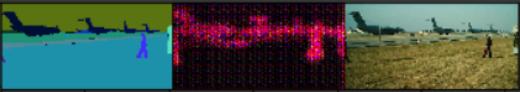
\includegraphics[width=10cm]{images/without-VGG}
  \end{center}
  \caption{不使用VGG损失训练集上生成的图片示例}
  \label{fig:without-VGG}
\end{figure}

之后,我又试着加上VGG损失,可以明显地看到生成器恢复了正常,结果如图\ref{fig:with-VGG}所示。因此,后面的实验和测试中,都是使用了VGG损失的。
\begin{figure}[H]
  \begin{center}
  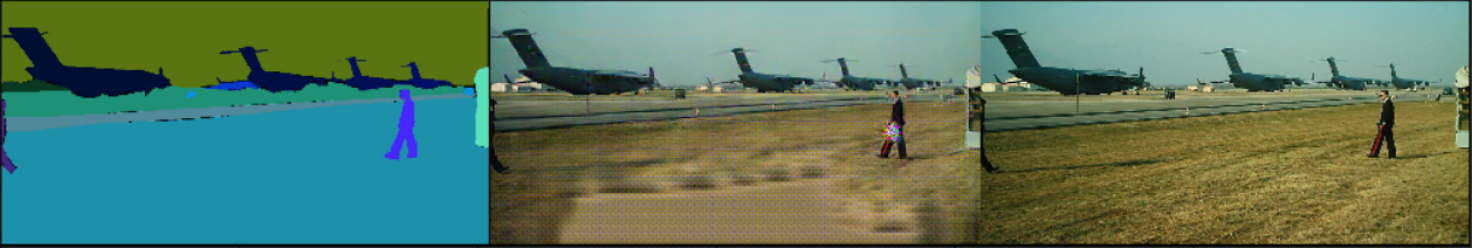
\includegraphics[width=10cm]{images/with-VGG}
  \end{center}
  \caption{使用了VGG损失训练集上生成的图片示例}
  \label{fig:with-VGG}
\end{figure}

VGG感知损失是基于VGG-19模型\cite{articleVGG}提出的,它是一个针对图像识别问题训练好的非常强大的神经网络模型。使用VGG损失意味着我们比较了
使用VGG模型从真实图片上提取的特征以及生成器生成过程中的图像特征。由于VGG十分强大,我们可以认为其提取的特征基本准确,这样一来,如果我们的
生成器生成的特征和真实图片的特征相似,那么最终的
结果也很有可能和真实图片相似。VGG损失的方法已经在风格迁移\cite{DBLP:journals/corr/JohnsonAL16}问题上大获成功。

不过,即使是使用了VGG损失,想要只用ADE20K数据集个别场景的数据就在测试集上取得好效果似乎不太现实。正如图\ref{fig:ADE20K-test}所示,模型
似乎遇到了过拟合的问题,即模型在训练集上表现非常好,但是在测试集上却表现糟糕。这很可能是由于训练数据不够导致的,比如说,在训练的时候,模型从来
没见到过一个人直接站在摄像头面前的情况,那么它自然不会知道这个人应该长什么样,这也就是为什么生成图片中都是马赛克了。之后,我又在Cityscapes中
做了实验,因为Cityscapes的所有图片都是都市街景这一类的场景,对于模型来说应该相对更容易学习。
\begin{figure}[H]
  \begin{center}
  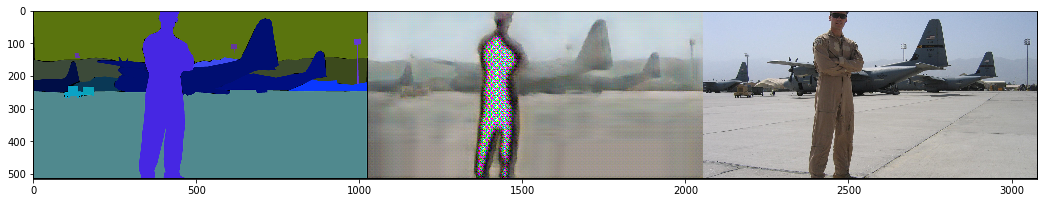
\includegraphics[width=10cm]{images/ade20k-test}
  \end{center}
  \caption{ADE20K空军基地测试集上生成图片示例}
  \label{fig:ADE20K-test}
\end{figure}

\subsubsection{Cityscapes数据集实验}

Cityscapes数据集上的实验是花时间最多的部分,尽管我只用了全部5000对数据中的3000对。对于局部强化器来说,训练一个周期就大概需要500秒的时间。下面
两张图片\ref{fig:Cityscapes-train} \ref{fig:Cityscapes-test}是全局生成器训练了500周期,局部强化器训练了200周期后的结果示例。我们依然
能看到一些过拟合的迹象,因为模型在训练集上的表现还是要远远强于测试集。训练时生成的图片和真实的相差无几,但是测试集的生成图片则是有很多模糊的地方,
看起来并没有那么真实。
\begin{figure}[H]
  \begin{center}
  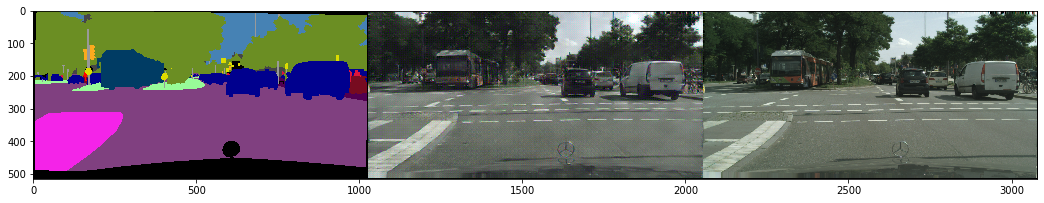
\includegraphics[width=14cm]{images/cityscapes-train}
  \end{center}
  \caption{Cityscapes数据集训练生成图片示例}
  \label{fig:Cityscapes-train}
\end{figure}

\begin{figure}[H]
  \begin{center}
  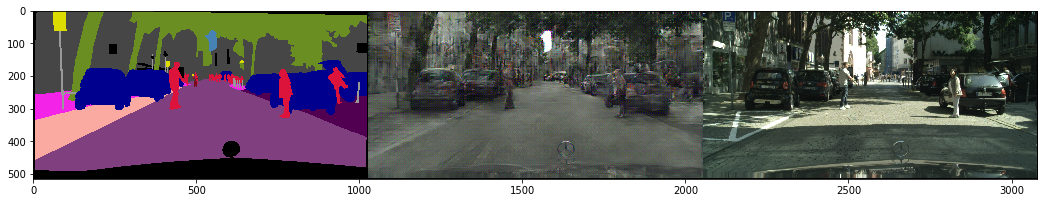
\includegraphics[width=14cm]{images/cityscapes-test}
  \end{center}
  \caption{Cityscapes数据集测试生成图片示例}
  \label{fig:Cityscapes-test}
\end{figure}

比较训练集和测试集的数据会发现测试的效果不如训练的效果。继续训练更多的周期或者调整超参数也不太可能解决这个问题,因为我们的模型已经能过很好地学习
训练集的数据了,所以这看上去更像是过拟合而不是欠拟合。增加训练的数据量是一个可行的办法,但是过长的训练时间也是一个大问题。我认为这一切的原因是
Cityscapes数据集包含了太多种类的物体,而且有些物体具有很复杂的纹理,这使得模型需要更多地训练图片去学习才能够不带有模糊地生成这些图像。所以,
我想的解决方案就是用一个像Cityscapes一样是单一场景,而且没有那么多种类的物体,物体纹理相对简单的数据集,Freiburg森林数据集刚好符合这些要求。

\subsubsection{基于Freiburg森林数据集的训练}

我们在\ref{sec:forest}中已经介绍过Freiburg森林数据集。首先我训练了200周期的全局生成器,从结果来看,尽管我们提高了生成器的学习速率,但是训练
依然很稳定,看起来是成功了。我追踪输出了每一个周期训练后全局生成器和辨别器的损失,如图\ref{fig:global-generator-loss}所示,看着是合理的。
\begin{figure}[H]
  \begin{center}
  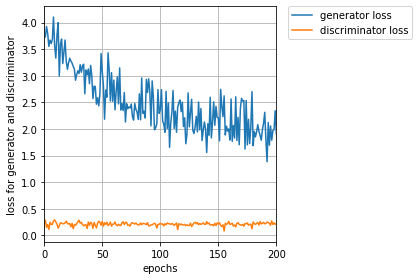
\includegraphics[width=8cm]{images/global-generator-loss}
  \end{center}
  \caption{训练中的全局生成器和辨别器的损失变化曲线图}
  \label{fig:global-generator-loss}
\end{figure}

全局生成器经过训练之后在测试阶段也可以生成不错的图片,不过,我们仔细查看图\ref{fig:global-generator-output}所示的结果,还是可以看到有一些
“噪点”,但是这个问题在我们训练一定周期的局部强化器后就没那么严重了。
\begin{figure}[H]
  \begin{center}
  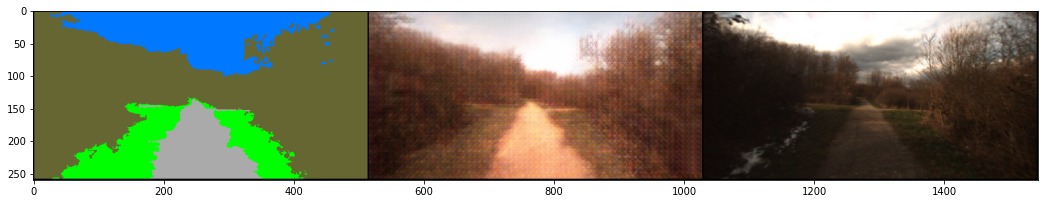
\includegraphics[width=14cm]{images/global-generator-output}
  \end{center}
  \caption{Pix2pixHD全局生成器测试阶段输出示例}
  \label{fig:global-generator-output}
\end{figure}

经过100个周期的局部强化器的训练(大约4-5小时),生成器就可以输出像图\ref{fig:local-enhancer-output}一样的高质量的图片了。由于局部强化器旨在
生成高分辨率的图像,所以之前“噪点”的问题看上去也不明显了。尽管某些局部仍然看起来有些模糊,但是考虑到有限的算力和训练时间,这样的图像质量是可以接受
的。所有的训练参数都和之前一样,训练也和全局生成器一样稳定,详见训练损失变化图\ref{fig:local-enhancer-loss}。

\begin{figure}[H]
  \begin{center}
  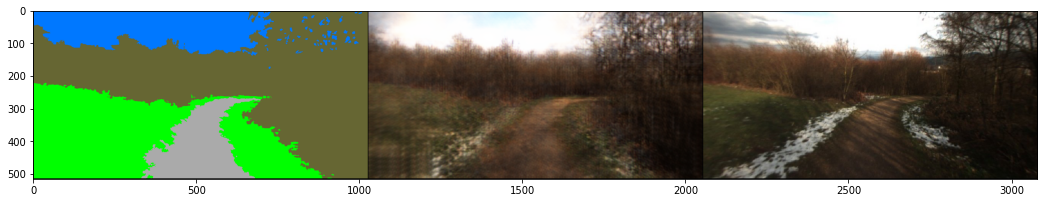
\includegraphics[width=14cm]{images/local-enhancer-output}
  \end{center}
  \caption{Pix2PixHD局部强化器测试阶段输出示例}
  \label{fig:local-enhancer-output}
\end{figure}

\begin{figure}[H]
  \begin{center}
  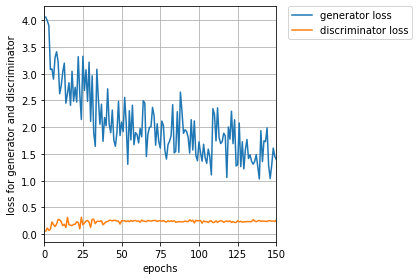
\includegraphics[width=8cm]{images/local-enhancer-loss}
  \end{center}
  \caption{训练中的局部强化器和辨别器的损失变化曲线图}
  \label{fig:local-enhancer-loss}
\end{figure}

\subsubsection{实验总结}

下表\ref{experimental results on Pix2pixHD}是Pix2pixHD的实验条件和对应结果,多次重复实验的结果也是一致的:
\begin{table}[H]
  \begin{center}
  \begin{tabular}{|l|l|l|l|l|}\hline\hline
  使用的数据集&是否使用VGG&训练是否稳定&训练集上效果&测试集上效果\\
  \hline
  ADE20K&否&是&不好&不好\\
  ADE20K&是&是&好&不好\\
  Cityscapes&是&是&好&不好\\
  Freiburg森林&是&是&好&好\\
  \hline\hline
  \end{tabular}
  \end{center}
  \caption{Pix2pixHD模型的实验结果总结}
  \label{experimental results on Pix2pixHD}
\end{table}

\subsection{SPADE模型实现}

SPADE是在Pix2pixHD之后提出的,目的是进一步提高图像翻译的质量。SPADE的论文给出了网络实现的诸多细节,所以实现起来并不是那么困难,另外,
由于SPADE借用了很多Pix2pixHD的思路,所以除了生成器之外,和Pix2pixHD的代码是通用的。

\subsubsection{生成器}

SPADE的生成器可以根据论文\cite{park2019SPADE}中“Additional Implementation Details”这一章节通过堆叠模块来搭建。SPADE网络的搭建
顺序应为:首先定义SPADE模块,然后使用SPADE模块去定义SPADE残差模块,最后在把SPADE残差模块整合进传统的生成对抗网络结构中去从而最终得到
SPADE生成器。值得注意的是,这个项目里,我们使用的图片的分辨率为$512\times256$,而不是原论文中的$256\times256$,所以,我们需要就输入
张量形状上做一点小改进,生成器大体的结构如图\ref{fig:SPADE-imp-generator}所示,具体的结构也可以查看附录中表的\ref{SPADE generator table}。

如图\ref{fig:SPADE-imp-generator}所示,整个生成图像过程的第一步是生成形如(1, 8192)的随机噪声(我们这里批大小设置为1),然后我们
改变这个张量的形状为(1024, 4, 2),之后,输入噪声将会通过7个SPADE残差模块处理,语义分割图的信息也会在此过程中读入,然后我们在将每个
残差的输出张量上采样2倍,最后通过一个卷积层和双曲正切激活函数将张量转化为图像。SPADE模块和SPADE残差模块的结构可以参考第二章的
图\ref{fig:SPADE-Block}和图\ref{fig:SPADE-ResBlock}。
\begin{figure}
  \begin{center}
  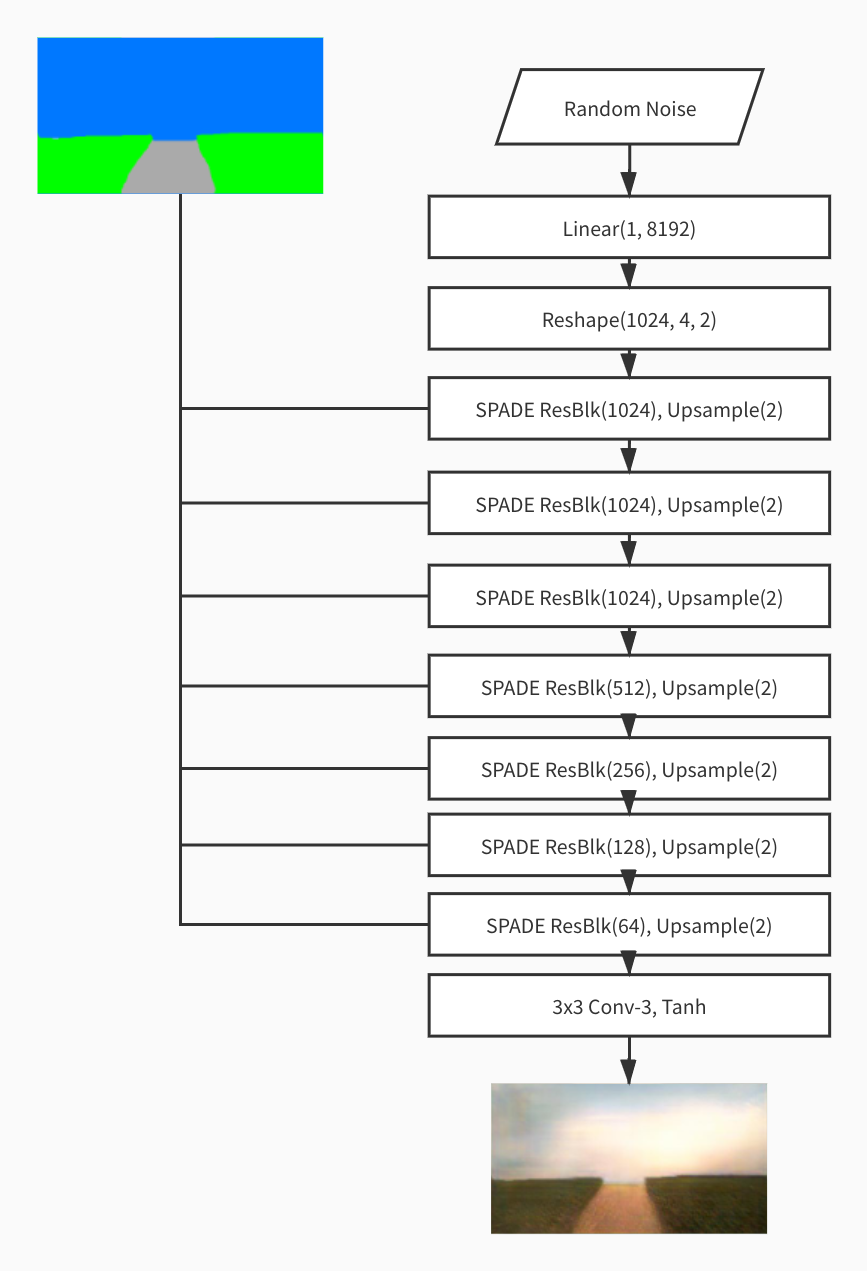
\includegraphics[width=8cm]{images/SPADE-imp-generator}
  \end{center}
  \caption{应用于Freiburg森林数据集的SPADE生成器结构}
  \label{fig:SPADE-imp-generator}
\end{figure}

\subsubsection{训练和结果}

因为只有生成器不一样,所以训练的配置也和Pix2pixHD的相同。我训练了SPADE生成器150个周期之后他就可以生成出像\ref{fig:SPADE-output}一样
的较为清晰的照片般的图片了。从损失变化曲线图\ref{fig:SPADE-loss}来看,SPADE模型的训练依然很稳定。另外,从
表\ref{experimental results on SPADE}我们不难看出,经过更多周期的训练,模型生成的图像质量也越来越高,在45个周期前提升更加明显,在那
之后,生成器的提高就很缓慢了。
\begin{figure}
  \begin{center}
  \includegraphics[width=14cm]{images/SPADE-output}
  \end{center}
  \caption{SPADE生成器测试阶段输出示例}
  \label{fig:SPADE-output}
\end{figure}
\begin{figure}
  \begin{center}
  \includegraphics[width=8cm]{images/SPADE-loss}
  \end{center}
  \caption{训练中的SPADE生成器损失变化曲线图}
  \label{fig:SPADE-loss}
\end{figure}

\begin{table}
  \begin{center}
  \begin{tabular}{|l|l|l|}\hline\hline
  训练周期数&生成器损失&测试集上的测试结果\\
  \hline
  1&3.118682861328125&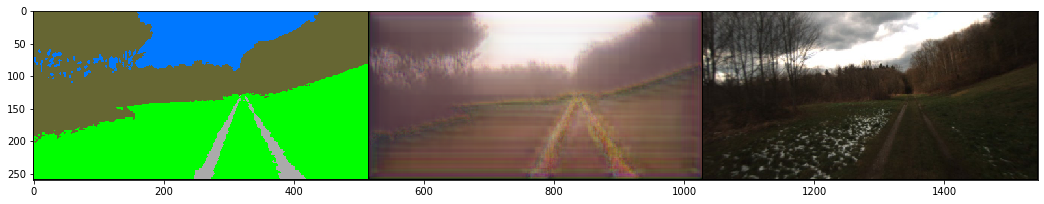
\includegraphics[width=8cm]{images/spade-epoch-1}\\
  15&2.3608477115631104&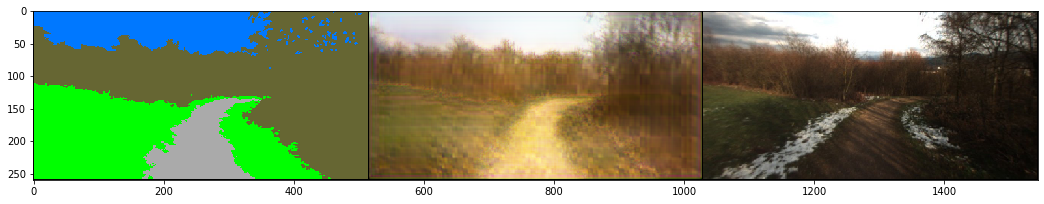
\includegraphics[width=8cm]{images/spade-epoch-15}\\
  30&2.2259953022003174&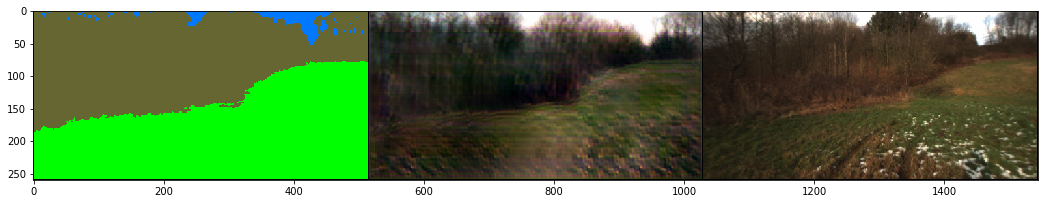
\includegraphics[width=8cm]{images/spade-epoch-30}\\
  45&1.8741878271102905&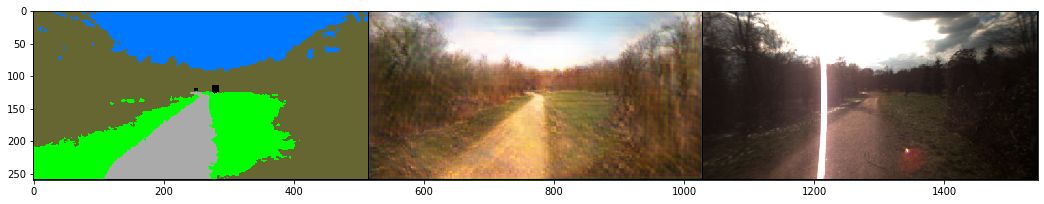
\includegraphics[width=8cm]{images/spade-epoch-45}\\
  60&1.6682815551757812&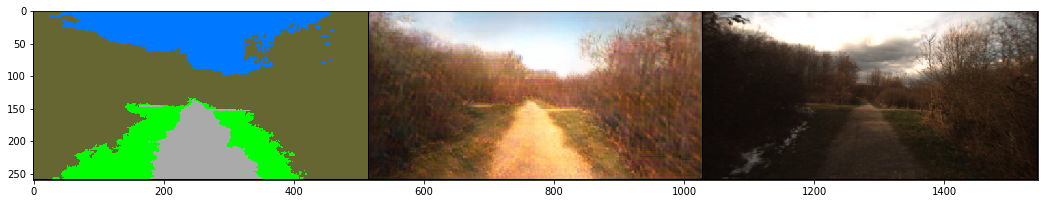
\includegraphics[width=8cm]{images/spade-epoch-60}\\
  75&1.5951969623565674&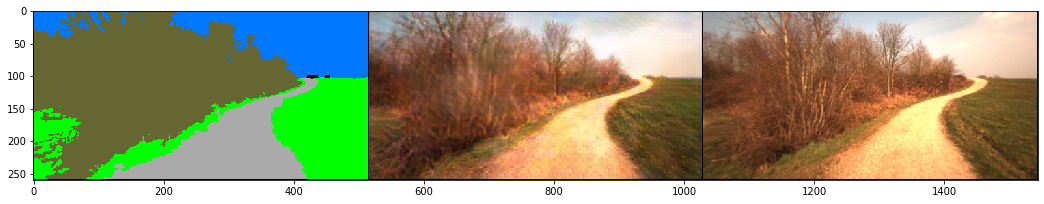
\includegraphics[width=8cm]{images/spade-epoch-75}\\
  150&1.4927189350128174&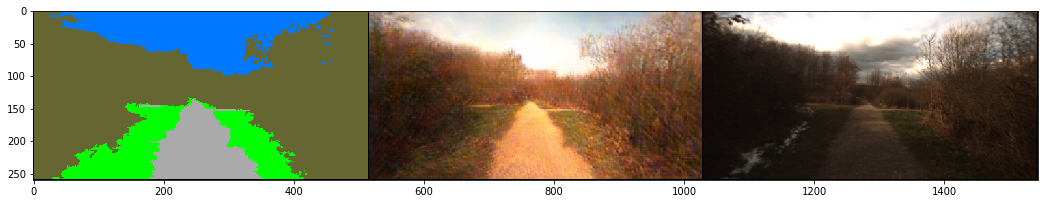
\includegraphics[width=8cm]{images/spade-epoch-150}\\
  \hline\hline
  \end{tabular}
  \end{center}
  \caption{SPADE模型的实验结果表格}
  \label{experimental results on SPADE}
\end{table}

\subsection{模型结果对比}

如果我们比较Pix2pixHD模型和SPADE模型的结果,我们可以发现SPADE模型有如下几点优势:
\begin{itemize}
  \item 图像更加清晰,没有“噪点”:尽管生成的图像并不是完全没有模糊,但是确实没有了Pix2pixHD中观察到的
  “噪点”现象。如果我们想要更高品质的生成结果,我们就需要投入更多的训练数据和更多的训练时间。
  \item 只需要训练一个生成器:当我实现这两个模型的时候,我觉得Pix2pixHD生成器的两个部分都需要训练是很烦的
  一件事,而且两个模型的训练时间加在一起甚至比一个复杂的模型花的时间更多。
  \item 实现风格迁移的可能性:由于在SPADE模型中,我们不再需要条件生成对抗网络的结构来读入语义分割图了,所以
  这部分的编码器可以替换为一个变分自动编码器来读入风格图片的信息以实现风格迁移的功能。这部分我没有来得及实现,
  具体的细节请参考章节\ref{sec:future work}。
\end{itemize}

然而Pix2pixHD模型依然可以称为是当下最先进模型之一,因为它提供了一个可以生成高分辨率图像的方法。SPADE模型或许也
可以生成更高分辨率的图像,然而SPADE模型需要占用更多的内存空间以及需要在测试阶段花费更长的时间才能完成图像翻译,
鉴于现在生成低分辨率图像SPADE都需要花上不短的时间,如果再追求高分辨率的话,可能就更慢了。

\section{总结与展望}
\subsection{项目规划和安排}

整个项目的开发分为4个部分:
\begin{enumerate}
  \item 阅读相关论文并做好相关知识和编程技术的积累:
  
  本项目主要参考的论文是Pix2pix\cite{pix2pix2016}, Pix2pixHD\cite{wang2018pix2pixHD}, SPADE\cite{park2019SPADE}这三篇, 
  另外我还花时间学习了如卷积神经网络、生成对抗网络、风格迁移等深度学习、计算机视觉相关的知识,以及写最终应用程序所需要用到的库,包括
  Pytorch、Flask等。
  \item 实现并训练图像翻译模型:
  
  这是整个毕业设计最困难的也是最花时间的部分,我想要实现两个当前最好的图像翻译模型,然而,在缺少大量的计算资源的Colab平台上想要像论文描述
  的那样训练出模型并不容易,比如说,SPADE的作者声称他们使用了8块英伟达V100的GPU训练了4天才达到论文中的效果,显然,就算不考虑Colab的断线
  问题,这也对我来说不现实。我想到的解决方案就是去掉耗费计算资源却对最终结果影响不大的组件并使用一个更加简单,体积小的数据集进行训练。
  \item 开发图形化界面: 
  
  这一部分主要是个软件工程的任务,由于在软件工程的课程上有过使用Java和Spring网页开发框架的经历,所以对我来说使用类似的Flask框架和Python
  开发一个网页应用并不是一个很复杂的任务。
  \item 写报告和录制短视频: 
  
  原本的计划是在3月16日的展示结束后就开始写报告,然而,由于新冠病毒的爆发,我买了3月22日的飞机票回国,之后我在西安集中隔离了14天,解除隔离
  后又回北京居家隔离了14天,所以实际开始全力投入写报告的时间比原计划晚了一些。最后按照华科计算机学院要求将英文报告翻译成中文。
\end{enumerate}
\begin{table}[H]
  \begin{center}
  \begin{tabular}{|l|l|l|l|}\hline\hline
  任务&计划时间安排&实际完成时间\\
  \hline
  相关知识技能准备&10/01 - 11/04&10/01 - 11/07\\
  训练神经网络&11/04 - 02/01&11/04 - 03/16\\
  开发展示应用程序&02/01 - 03/02&11/04 - 03/16\\
  报告和短视频&03/16 - 04/28&04/06 - 05/05\\
  英文报告翻译&05/12 - 05/30&05/12 - 05/30\\
  \hline\hline
  \end{tabular}
  \end{center}
  \caption{毕业设计规划时间表}
  \label{milestones table}
\end{table}

上表\ref{milestones table}展示了整个项目的任务表、计划安排时间表以及实际的完成情况。有几件事并没能按照最开始的计划完成,比如,制定计划的时候
开题演讲还没出时间安排,所以我开始训练神经网络的工作就从11月7日演讲结束了才开始,除此之外,由于在训练的过程中有很多的时间都用在等待训练结果上了,
所以实际操作的时候我将图形界面的开发和训练模型的工作合在一起做,我认为这样可以更加充分的利用时间。最后的报告阶段,由于新冠病毒爆发,我没能按原计划
完成报告,但是好在截止日期也一样完成了。

\subsection{后续工作}
\label{sec:future work}

由于算力和时间有限,我没能够实现两个当下最先进模型论文中提到的所有内容,这些内容包括:
\begin{itemize}
  \item Pix2pixHD论文中使用的实例轮廓图(Instance Map):
  
  在语义分割图中,每一种像素的数值代表了一类的物体,但是分割图并不会区分同一类物体的边界,例如,如果有两辆汽车紧挨在一起,
  我们并不能从语义分割图中看出来这两辆汽车的界线。而使用了轮廓图之后,我们便可以给每一个物体标上一个独有的ID值以此识别出
  每一个物体,这样模型就能够更好地生成物体和物体边界部分的图像了。
  \begin{figure}[H]
      \begin{center}
      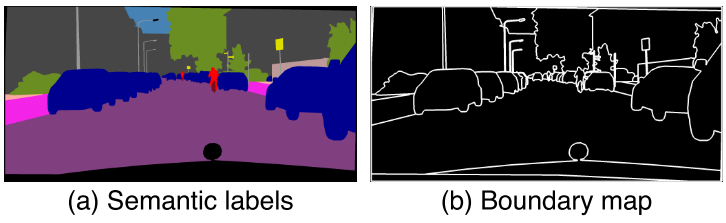
\includegraphics[width=8cm]{images/instance-map}
      \end{center}
      \caption{语义分割图(a) VS. 实例轮廓图(b)}
      \label{fig:instance-map}
  \end{figure}
  \item SPADE论文中使用的变分自动编码器
  
  正如第二章中介绍过的一样,SPADE去掉了条件生成网络中必备的针对语义分割图输入信息的编码器,所以SPADE模型可以使用一个用于
  风格迁移的变分自动编码器。这个编码器使用基层卷积神经网络将输入的风格图片转化为一个平均向量$\mu$,一个方差向量$\sigma$,
  这两个值将会用来计算最终输入到生成器的随机噪声,这样噪声中就包含了风格图片的信息。使用变分自动编码器需要另外单独训练。
  \item 基准数据集
  
  目前有几个现成的专门给图像翻译和语义分割训练使用的基准数据集,包括Cityscapes \cite{Cordts2016Cityscapes}, 
  ADE20K \cite{zhou2017scene}等。这些数据集相比我使用的数据集提供了更多的训练数据,如果能够完成这些数据集的测试,那么
  就能够证明这个模型的结构可以适用于如包含更多种类物体(Cityscapes数据集含有20种物体)或多种类别(ADE20K包含了机场、画廊等)
  等更加复杂的场景。然而,使用这些数据集训练需要更多的算力和更长的训练时间。
  \item 超参数搜索
  
  如果我们能确定每个模型的最好的超参数就更加理想了,但是进行超参数搜索需要重复训练很多次模型(每次训练可能都需要一天以上的时间)。
  如果想要这么做的话,或许需要一些启发式的搜索方式,因为想要遍历完所有的超参数组合显然是不可能的。
\end{itemize}

\subsection{总结与结论}

本毕业设计完成了图像翻译这一话题的文献综述,在算力有限的情况下实现了两个当下最先进的图像翻译模型,并比较了两者的优劣。所有的实验细节
都记录在了jupyter notebook中,而所有实现的模型也都包含在了一个带有图形化界面的网页应用程序中,这样一来,就算是不熟悉这一领域的人也
可以方便地查看实验的过程和结果,而没有机器学习和编程经验的人也可以通过本毕业设计的网页程序体验图像翻译的乐趣。

在开发和研究这个项目的过程中,我不但学到了很多有关深度学习和图像翻译的知识,而且提升了我的自学能力,一开始,我只是知道一些神经网络的基本
概念,后来我通过网络了解了卷积神经网络是如何解决这些计算机视觉相关的复杂问题的,以及如何使用深度学习框架搭建简单的卷积神经网络。为了了解
图像翻译,我读了几篇相关的论文,这些论文的新鲜观点一开始不是很容易理解,不过在一些博客和YouTube视频的讲解的帮助下还是基本上都明白了。
除了这些之外,我也实践了如何将机器学习的模型放到如网页应用程序这样的应用程序中运行。

在我看来,即使现在的这些先进的模型已经十分强大,作为一个原型产品来说绰绰有余,但是距离商用还是有一定距离的。首先,这些方法虽然效果很好,但是
对于计算资源的消耗还是过大,比如,想要重现论文中的风景画模型,我需要8块英伟达V100的GPU一起训练几天,但是对于大部分想要训练一个生成特定类型
图像的用户来说都不具备如此强大的算力。另外一个问题就是这种模型的数据集并不像看上去那么容易找到,比如说,想要帮助设计师设计新奇的产品,就很难
找到“新奇”产品的数据集用于训练。

\begin{thankpage}

首先我要感谢华中科技大学计算机学院给予我的和英国曼彻斯特大学计算机学院的2+2的出国交流机会,
英国的两年学习生活使我收益良多,我收获的不仅仅是本科的文凭,我还体验了英国的生活文化,结识了来自世界各地的朋友,
了解了国外大学的教学科研体系等。

这个毕业设计是在曼彻斯特大学交换期间完成的,我十分感激我的导师Angelo Cangelosi教授,他在本项目的研发过程中的
耐心与指导,以及提出的各种建设性意见都是我最终得以完成此毕业设计的关键。

除此之外,我非常感谢大学四年里所有的老师、同学、朋友,还有我的家人对我的帮助、鼓励和支持,没有你们,这一切都是不可能如此顺利。

最后,我要感谢本次新冠疫情期间帮助过我的机场工作人员、医护人员、酒店工作人员等,多亏了您们的鼎力相助,我才能够平安顺利地回国回家。

\end{thankpage}

\nocite{*}

\bibliography{report}

\appendix
\section{附录:模型概述信息}
本附录包含了项目实现的两个生成器和一个辨别器神经网络的模型概述信息,由微软的tensorwatch开源软件生成。
具体的代码实现将会开源至我的\href{https://github.com/williamlwclwc}{GitHub}. 

\textbf{Pix2pixHD生成器结构概述信息}
\begin{longtable}{llll}
    \toprule
                        module name &        input shape &       output\_shape &  parameters \\
    \midrule
                    model\_global.0 &   (1, 3, 256, 128) &   (1, 3, 262, 134) &           0 \\
                    model\_global.1 &   (1, 3, 262, 134) &  (1, 64, 256, 128) &       9,472 \\
                    model\_global.2 &  (1, 64, 256, 128) &  (1, 64, 256, 128) &         128 \\
                    model\_global.3 &  (1, 64, 256, 128) &  (1, 64, 256, 128) &           0 \\
                    model\_global.4 &  (1, 64, 256, 128) &  (1, 128, 128, 64) &      73,856 \\
                    model\_global.5 &  (1, 128, 128, 64) &  (1, 128, 128, 64) &         256 \\
                    model\_global.6 &  (1, 128, 128, 64) &  (1, 128, 128, 64) &           0 \\
                    model\_global.7 &  (1, 128, 128, 64) &   (1, 256, 64, 32) &     295,168 \\
                    model\_global.8 &   (1, 256, 64, 32) &   (1, 256, 64, 32) &         512 \\
                    model\_global.9 &   (1, 256, 64, 32) &   (1, 256, 64, 32) &           0 \\
                    model\_global.10 &   (1, 256, 64, 32) &   (1, 512, 32, 16) &   1,180,160 \\
                    model\_global.11 &   (1, 512, 32, 16) &   (1, 512, 32, 16) &       1,024 \\
                    model\_global.12 &   (1, 512, 32, 16) &   (1, 512, 32, 16) &           0 \\
        model\_global.13.conv\_block.0 &   (1, 512, 32, 16) &   (1, 512, 34, 18) &           0 \\
        model\_global.13.conv\_block.1 &   (1, 512, 34, 18) &   (1, 512, 32, 16) &   2,359,808 \\
        model\_global.13.conv\_block.2 &   (1, 512, 32, 16) &   (1, 512, 32, 16) &       1,024 \\
        model\_global.13.conv\_block.3 &   (1, 512, 32, 16) &   (1, 512, 32, 16) &           0 \\
        model\_global.13.conv\_block.4 &   (1, 512, 32, 16) &   (1, 512, 34, 18) &           0 \\
        model\_global.13.conv\_block.5 &   (1, 512, 34, 18) &   (1, 512, 32, 16) &   2,359,808 \\
        model\_global.13.conv\_block.6 &   (1, 512, 32, 16) &   (1, 512, 32, 16) &       1,024 \\
        model\_global.14.conv\_block.0 &   (1, 512, 32, 16) &   (1, 512, 34, 18) &           0 \\
        model\_global.14.conv\_block.1 &   (1, 512, 34, 18) &   (1, 512, 32, 16) &   2,359,808 \\
        model\_global.14.conv\_block.2 &   (1, 512, 32, 16) &   (1, 512, 32, 16) &       1,024 \\
        model\_global.14.conv\_block.3 &   (1, 512, 32, 16) &   (1, 512, 32, 16) &           0 \\
        model\_global.14.conv\_block.4 &   (1, 512, 32, 16) &   (1, 512, 34, 18) &           0 \\
        model\_global.14.conv\_block.5 &   (1, 512, 34, 18) &   (1, 512, 32, 16) &   2,359,808 \\
        model\_global.14.conv\_block.6 &   (1, 512, 32, 16) &   (1, 512, 32, 16) &       1,024 \\
        model\_global.15.conv\_block.0 &   (1, 512, 32, 16) &   (1, 512, 34, 18) &           0 \\
        model\_global.15.conv\_block.1 &   (1, 512, 34, 18) &   (1, 512, 32, 16) &   2,359,808 \\
        model\_global.15.conv\_block.2 &   (1, 512, 32, 16) &   (1, 512, 32, 16) &       1,024 \\
        model\_global.15.conv\_block.3 &   (1, 512, 32, 16) &   (1, 512, 32, 16) &           0 \\
        model\_global.15.conv\_block.4 &   (1, 512, 32, 16) &   (1, 512, 34, 18) &           0 \\
        model\_global.15.conv\_block.5 &   (1, 512, 34, 18) &   (1, 512, 32, 16) &   2,359,808 \\
        model\_global.15.conv\_block.6 &   (1, 512, 32, 16) &   (1, 512, 32, 16) &       1,024 \\
        model\_global.16.conv\_block.0 &   (1, 512, 32, 16) &   (1, 512, 34, 18) &           0 \\
        model\_global.16.conv\_block.1 &   (1, 512, 34, 18) &   (1, 512, 32, 16) &   2,359,808 \\
        model\_global.16.conv\_block.2 &   (1, 512, 32, 16) &   (1, 512, 32, 16) &       1,024 \\
        model\_global.16.conv\_block.3 &   (1, 512, 32, 16) &   (1, 512, 32, 16) &           0 \\
        model\_global.16.conv\_block.4 &   (1, 512, 32, 16) &   (1, 512, 34, 18) &           0 \\
        model\_global.16.conv\_block.5 &   (1, 512, 34, 18) &   (1, 512, 32, 16) &   2,359,808 \\
        model\_global.16.conv\_block.6 &   (1, 512, 32, 16) &   (1, 512, 32, 16) &       1,024 \\
        model\_global.17.conv\_block.0 &   (1, 512, 32, 16) &   (1, 512, 34, 18) &           0 \\
        model\_global.17.conv\_block.1 &   (1, 512, 34, 18) &   (1, 512, 32, 16) &   2,359,808 \\
        model\_global.17.conv\_block.2 &   (1, 512, 32, 16) &   (1, 512, 32, 16) &       1,024 \\
        model\_global.17.conv\_block.3 &   (1, 512, 32, 16) &   (1, 512, 32, 16) &           0 \\
        model\_global.17.conv\_block.4 &   (1, 512, 32, 16) &   (1, 512, 34, 18) &           0 \\
        model\_global.17.conv\_block.5 &   (1, 512, 34, 18) &   (1, 512, 32, 16) &   2,359,808 \\
        model\_global.17.conv\_block.6 &   (1, 512, 32, 16) &   (1, 512, 32, 16) &       1,024 \\
        model\_global.18.conv\_block.0 &   (1, 512, 32, 16) &   (1, 512, 34, 18) &           0 \\
        model\_global.18.conv\_block.1 &   (1, 512, 34, 18) &   (1, 512, 32, 16) &   2,359,808 \\
        model\_global.18.conv\_block.2 &   (1, 512, 32, 16) &   (1, 512, 32, 16) &       1,024 \\
        model\_global.18.conv\_block.3 &   (1, 512, 32, 16) &   (1, 512, 32, 16) &           0 \\
        model\_global.18.conv\_block.4 &   (1, 512, 32, 16) &   (1, 512, 34, 18) &           0 \\
        model\_global.18.conv\_block.5 &   (1, 512, 34, 18) &   (1, 512, 32, 16) &   2,359,808 \\
        model\_global.18.conv\_block.6 &   (1, 512, 32, 16) &   (1, 512, 32, 16) &       1,024 \\
                    model\_global.19 &   (1, 512, 32, 16) &   (1, 256, 64, 32) &   1,179,904 \\
                    model\_global.20 &   (1, 256, 64, 32) &   (1, 256, 64, 32) &         512 \\
                    model\_global.21 &   (1, 256, 64, 32) &   (1, 256, 64, 32) &           0 \\
                    model\_global.22 &   (1, 256, 64, 32) &  (1, 128, 128, 64) &     295,040 \\
                    model\_global.23 &  (1, 128, 128, 64) &  (1, 128, 128, 64) &         256 \\
                    model\_global.24 &  (1, 128, 128, 64) &  (1, 128, 128, 64) &           0 \\
                    model\_global.25 &  (1, 128, 128, 64) &  (1, 64, 256, 128) &      73,792 \\
                    model\_global.26 &  (1, 64, 256, 128) &  (1, 64, 256, 128) &         128 \\
                    model\_global.27 &  (1, 64, 256, 128) &  (1, 64, 256, 128) &           0 \\
                    model\_global.28 &                 [] &                 [] &           0 \\
                    model\_global.29 &                 [] &                 [] &           0 \\
                    model\_global.30 &                 [] &                 [] &           0 \\
                        downsample &   (1, 3, 512, 256) &   (1, 3, 256, 128) &           0 \\
                    le\_downsample.0 &   (1, 3, 512, 256) &   (1, 3, 518, 262) &           0 \\
                    le\_downsample.1 &   (1, 3, 518, 262) &  (1, 32, 512, 256) &       4,736 \\
                    le\_downsample.2 &  (1, 32, 512, 256) &  (1, 32, 512, 256) &          64 \\
                    le\_downsample.3 &  (1, 32, 512, 256) &  (1, 32, 512, 256) &           0 \\
                    le\_downsample.4 &  (1, 32, 512, 256) &  (1, 64, 256, 128) &      18,496 \\
                    le\_downsample.5 &  (1, 64, 256, 128) &  (1, 64, 256, 128) &         128 \\
                    le\_downsample.6 &  (1, 64, 256, 128) &  (1, 64, 256, 128) &           0 \\
        le\_upsample.0.conv\_block.0 &  (1, 64, 256, 128) &  (1, 64, 258, 130) &           0 \\
        le\_upsample.0.conv\_block.1 &  (1, 64, 258, 130) &  (1, 64, 256, 128) &      36,928 \\
        le\_upsample.0.conv\_block.2 &  (1, 64, 256, 128) &  (1, 64, 256, 128) &         128 \\
        le\_upsample.0.conv\_block.3 &  (1, 64, 256, 128) &  (1, 64, 256, 128) &           0 \\
        le\_upsample.0.conv\_block.4 &  (1, 64, 256, 128) &  (1, 64, 258, 130) &           0 \\
        le\_upsample.0.conv\_block.5 &  (1, 64, 258, 130) &  (1, 64, 256, 128) &      36,928 \\
        le\_upsample.0.conv\_block.6 &  (1, 64, 256, 128) &  (1, 64, 256, 128) &         128 \\
        le\_upsample.1.conv\_block.0 &  (1, 64, 256, 128) &  (1, 64, 258, 130) &           0 \\
        le\_upsample.1.conv\_block.1 &  (1, 64, 258, 130) &  (1, 64, 256, 128) &      36,928 \\
        le\_upsample.1.conv\_block.2 &  (1, 64, 256, 128) &  (1, 64, 256, 128) &         128 \\
        le\_upsample.1.conv\_block.4 &  (1, 64, 256, 128) &  (1, 64, 258, 130) &           0 \\
        le\_upsample.1.conv\_block.5 &  (1, 64, 258, 130) &  (1, 64, 256, 128) &      36,928 \\
        le\_upsample.1.conv\_block.6 &  (1, 64, 256, 128) &  (1, 64, 256, 128) &         128 \\
        le\_upsample.2.conv\_block.0 &  (1, 64, 256, 128) &  (1, 64, 258, 130) &           0 \\
        le\_upsample.2.conv\_block.1 &  (1, 64, 258, 130) &  (1, 64, 256, 128) &      36,928 \\
        le\_upsample.2.conv\_block.2 &  (1, 64, 256, 128) &  (1, 64, 256, 128) &         128 \\
        le\_upsample.2.conv\_block.4 &  (1, 64, 256, 128) &  (1, 64, 258, 130) &           0 \\
        le\_upsample.2.conv\_block.5 &  (1, 64, 258, 130) &  (1, 64, 256, 128) &      36,928 \\
        le\_upsample.2.conv\_block.6 &  (1, 64, 256, 128) &  (1, 64, 256, 128) &         128 \\
                    le\_upsample.3 &  (1, 64, 256, 128) &  (1, 32, 512, 256) &      18,464 \\
                    le\_upsample.4 &  (1, 32, 512, 256) &  (1, 32, 512, 256) &          64 \\
                    le\_upsample.5 &  (1, 32, 512, 256) &  (1, 32, 512, 256) &           0 \\
                    le\_upsample.6 &  (1, 32, 512, 256) &  (1, 32, 518, 262) &           0 \\
                    le\_upsample.7 &  (1, 32, 518, 262) &   (1, 3, 512, 256) &       4,707 \\
                    le\_upsample.8 &   (1, 3, 512, 256) &   (1, 3, 512, 256) &           0 \\
                            Model &   [1, 3, 512, 256] &   (1, 3, 512, 256) &  31,709,187 \\
    \bottomrule
    \caption{由tensorwatch生成的Pix2pixHD生成器模型概述信息}
    \label{Pix2pixHD generator table}
\end{longtable}  
    
\textbf{辨别器的模型结构概述信息}
\begin{table}[H]
    \begin{tabular}{llll}
        \toprule
        module name &        input shape &       output shape & parameters \\
        \midrule
        downsample &   (1, 6, 256, 128) &    (1, 6, 128, 64) &          0 \\
        layer0.0 &    (1, 6, 128, 64) &    (1, 64, 65, 33) &      6,208 \\
        layer0.1 &    (1, 64, 65, 33) &    (1, 64, 65, 33) &          0 \\
        layer0.2 &    (1, 64, 65, 33) &   (1, 128, 33, 17) &    131,200 \\
        layer0.3 &   (1, 128, 33, 17) &   (1, 128, 33, 17) &        256 \\
        layer0.4 &   (1, 128, 33, 17) &   (1, 128, 33, 17) &          0 \\
        layer0.5 &   (1, 128, 33, 17) &    (1, 256, 17, 9) &    524,544 \\
        layer0.6 &    (1, 256, 17, 9) &    (1, 256, 17, 9) &        512 \\
        layer0.7 &    (1, 256, 17, 9) &    (1, 256, 17, 9) &          0 \\
        layer0.8 &    (1, 256, 17, 9) &   (1, 512, 18, 10) &  2,097,664 \\
        layer0.9 &   (1, 512, 18, 10) &   (1, 512, 18, 10) &      1,024 \\
        layer0.10 &   (1, 512, 18, 10) &   (1, 512, 18, 10) &          0 \\
        layer0.11 &   (1, 512, 18, 10) &     (1, 1, 19, 11) &      8,193 \\
        layer1.0 &   (1, 6, 256, 128) &   (1, 64, 129, 65) &      6,208 \\
        layer1.1 &   (1, 64, 129, 65) &   (1, 64, 129, 65) &          0 \\
        layer1.2 &   (1, 64, 129, 65) &   (1, 128, 65, 33) &    131,200 \\
        layer1.3 &   (1, 128, 65, 33) &   (1, 128, 65, 33) &        256 \\
        layer1.4 &   (1, 128, 65, 33) &   (1, 128, 65, 33) &          0 \\
        layer1.5 &   (1, 128, 65, 33) &   (1, 256, 33, 17) &    524,544 \\
        layer1.6 &   (1, 256, 33, 17) &   (1, 256, 33, 17) &        512 \\
        layer1.7 &   (1, 256, 33, 17) &   (1, 256, 33, 17) &          0 \\
        layer1.8 &   (1, 256, 33, 17) &   (1, 512, 34, 18) &  2,097,664 \\
        layer1.9 &   (1, 512, 34, 18) &   (1, 512, 34, 18) &      1,024 \\
        layer1.10 &   (1, 512, 34, 18) &   (1, 512, 34, 18) &          0 \\
        layer1.11 &   (1, 512, 34, 18) &     (1, 1, 35, 19) &      8,193 \\
        layer2.0 &   (1, 6, 512, 256) &  (1, 64, 257, 129) &      6,208 \\
        layer2.1 &  (1, 64, 257, 129) &  (1, 64, 257, 129) &          0 \\
        layer2.2 &  (1, 64, 257, 129) &  (1, 128, 129, 65) &    131,200 \\
        layer2.3 &  (1, 128, 129, 65) &  (1, 128, 129, 65) &        256 \\
        layer2.4 &  (1, 128, 129, 65) &  (1, 128, 129, 65) &          0 \\
        layer2.5 &  (1, 128, 129, 65) &   (1, 256, 65, 33) &    524,544 \\
        layer2.6 &   (1, 256, 65, 33) &   (1, 256, 65, 33) &        512 \\
        layer2.7 &   (1, 256, 65, 33) &   (1, 256, 65, 33) &          0 \\
        layer2.8 &   (1, 256, 65, 33) &   (1, 512, 66, 34) &  2,097,664 \\
        layer2.9 &   (1, 512, 66, 34) &   (1, 512, 66, 34) &      1,024 \\
        layer2.10 &   (1, 512, 66, 34) &   (1, 512, 66, 34) &          0 \\
        layer2.11 &   (1, 512, 66, 34) &     (1, 1, 67, 35) &      8,193 \\
            Model &   [1, 6, 512, 256] &     (1, 1, 67, 35) &  8,308,803 \\
        \bottomrule
    \end{tabular}
    \caption{由tensorwatch生成的辨别器模型概述信息}
    \label{Pix2pixHD discriminator table}
\end{table}
    
\textbf{SPADE模型的生成器模型概述信息}
\begin{longtable}{llll}
    \toprule
                            module name &         input shape &        output shape &   parameters \\
    \midrule
                                    fc &            (1, 256) &           (1, 8192) &    2,105,344 \\
        spadeRes0.spade0.param\_free\_norm &     (1, 1024, 4, 2) &     (1, 1024, 4, 2) &            0 \\
            spadeRes0.spade0.shared\_net.0 &        (1, 3, 4, 2) &      (1, 128, 4, 2) &        3,584 \\
            spadeRes0.spade0.shared\_net.1 &      (1, 128, 4, 2) &      (1, 128, 4, 2) &            0 \\
                spadeRes0.spade0.gamma &      (1, 128, 4, 2) &     (1, 1024, 4, 2) &    1,180,672 \\
                    spadeRes0.spade0.beta &      (1, 128, 4, 2) &     (1, 1024, 4, 2) &    1,180,672 \\
                        spadeRes0.conv0 &     (1, 1024, 4, 2) &     (1, 1024, 4, 2) &    9,438,208 \\
                        spadeRes0.relu0 &     (1, 1024, 4, 2) &     (1, 1024, 4, 2) &            0 \\
        spadeRes0.spade1.param\_free\_norm &     (1, 1024, 4, 2) &     (1, 1024, 4, 2) &            0 \\
            spadeRes0.spade1.shared\_net.0 &        (1, 3, 4, 2) &      (1, 128, 4, 2) &        3,584 \\
            spadeRes0.spade1.shared\_net.1 &      (1, 128, 4, 2) &      (1, 128, 4, 2) &            0 \\
                spadeRes0.spade1.gamma &      (1, 128, 4, 2) &     (1, 1024, 4, 2) &    1,180,672 \\
                    spadeRes0.spade1.beta &      (1, 128, 4, 2) &     (1, 1024, 4, 2) &    1,180,672 \\
                        spadeRes0.conv1 &     (1, 1024, 4, 2) &     (1, 1024, 4, 2) &    9,438,208 \\
                        spadeRes0.relu1 &     (1, 1024, 4, 2) &     (1, 1024, 4, 2) &            0 \\
    spadeRes0.spade\_skip.param\_free\_norm &     (1, 1024, 4, 2) &     (1, 1024, 4, 2) &            0 \\
        spadeRes0.spade\_skip.shared\_net.0 &        (1, 3, 4, 2) &      (1, 128, 4, 2) &        3,584 \\
        spadeRes0.spade\_skip.shared\_net.1 &      (1, 128, 4, 2) &      (1, 128, 4, 2) &            0 \\
            spadeRes0.spade\_skip.gamma &      (1, 128, 4, 2) &     (1, 1024, 4, 2) &    1,180,672 \\
                spadeRes0.spade\_skip.beta &      (1, 128, 4, 2) &     (1, 1024, 4, 2) &    1,180,672 \\
                    spadeRes0.conv\_skip &     (1, 1024, 4, 2) &     (1, 1024, 4, 2) &    1,048,576 \\
                    spadeRes0.relu\_skip &     (1, 1024, 4, 2) &     (1, 1024, 4, 2) &            0 \\
        spadeRes1.spade0.param\_free\_norm &     (1, 1024, 8, 4) &     (1, 1024, 8, 4) &            0 \\
            spadeRes1.spade0.shared\_net.0 &        (1, 3, 8, 4) &      (1, 128, 8, 4) &        3,584 \\
            spadeRes1.spade0.shared\_net.1 &      (1, 128, 8, 4) &      (1, 128, 8, 4) &            0 \\
                spadeRes1.spade0.gamma &      (1, 128, 8, 4) &     (1, 1024, 8, 4) &    1,180,672 \\
                    spadeRes1.spade0.beta &      (1, 128, 8, 4) &     (1, 1024, 8, 4) &    1,180,672 \\
                        spadeRes1.conv0 &     (1, 1024, 8, 4) &     (1, 1024, 8, 4) &    9,438,208 \\
                        spadeRes1.relu0 &     (1, 1024, 8, 4) &     (1, 1024, 8, 4) &            0 \\
        spadeRes1.spade1.param\_free\_norm &     (1, 1024, 8, 4) &     (1, 1024, 8, 4) &            0 \\
            spadeRes1.spade1.shared\_net.0 &        (1, 3, 8, 4) &      (1, 128, 8, 4) &        3,584 \\
            spadeRes1.spade1.shared\_net.1 &      (1, 128, 8, 4) &      (1, 128, 8, 4) &            0 \\
                spadeRes1.spade1.gamma &      (1, 128, 8, 4) &     (1, 1024, 8, 4) &    1,180,672 \\
                    spadeRes1.spade1.beta &      (1, 128, 8, 4) &     (1, 1024, 8, 4) &    1,180,672 \\
                        spadeRes1.conv1 &     (1, 1024, 8, 4) &     (1, 1024, 8, 4) &    9,438,208 \\
                        spadeRes1.relu1 &     (1, 1024, 8, 4) &     (1, 1024, 8, 4) &            0 \\
    spadeRes1.spade\_skip.param\_free\_norm &     (1, 1024, 8, 4) &     (1, 1024, 8, 4) &            0 \\
        spadeRes1.spade\_skip.shared\_net.0 &        (1, 3, 8, 4) &      (1, 128, 8, 4) &        3,584 \\
        spadeRes1.spade\_skip.shared\_net.1 &      (1, 128, 8, 4) &      (1, 128, 8, 4) &            0 \\
            spadeRes1.spade\_skip.gamma &      (1, 128, 8, 4) &     (1, 1024, 8, 4) &    1,180,672 \\
                spadeRes1.spade\_skip.beta &      (1, 128, 8, 4) &     (1, 1024, 8, 4) &    1,180,672 \\
                    spadeRes1.conv\_skip &     (1, 1024, 8, 4) &     (1, 1024, 8, 4) &    1,048,576 \\
                    spadeRes1.relu\_skip &     (1, 1024, 8, 4) &     (1, 1024, 8, 4) &            0 \\
        spadeRes2.spade0.param\_free\_norm &    (1, 1024, 16, 8) &    (1, 1024, 16, 8) &            0 \\
            spadeRes2.spade0.shared\_net.0 &       (1, 3, 16, 8) &     (1, 128, 16, 8) &        3,584 \\
            spadeRes2.spade0.shared\_net.1 &     (1, 128, 16, 8) &     (1, 128, 16, 8) &            0 \\
                spadeRes2.spade0.gamma &     (1, 128, 16, 8) &    (1, 1024, 16, 8) &    1,180,672 \\
                    spadeRes2.spade0.beta &     (1, 128, 16, 8) &    (1, 1024, 16, 8) &    1,180,672 \\
                        spadeRes2.conv0 &    (1, 1024, 16, 8) &    (1, 1024, 16, 8) &    9,438,208 \\
                        spadeRes2.relu0 &    (1, 1024, 16, 8) &    (1, 1024, 16, 8) &            0 \\
        spadeRes2.spade1.param\_free\_norm &    (1, 1024, 16, 8) &    (1, 1024, 16, 8) &            0 \\
            spadeRes2.spade1.shared\_net.0 &       (1, 3, 16, 8) &     (1, 128, 16, 8) &        3,584 \\
            spadeRes2.spade1.shared\_net.1 &     (1, 128, 16, 8) &     (1, 128, 16, 8) &            0 \\
                spadeRes2.spade1.gamma &     (1, 128, 16, 8) &    (1, 1024, 16, 8) &    1,180,672 \\
                    spadeRes2.spade1.beta &     (1, 128, 16, 8) &    (1, 1024, 16, 8) &    1,180,672 \\
                        spadeRes2.conv1 &    (1, 1024, 16, 8) &    (1, 1024, 16, 8) &    9,438,208 \\
                        spadeRes2.relu1 &    (1, 1024, 16, 8) &    (1, 1024, 16, 8) &            0 \\
    spadeRes2.spade\_skip.param\_free\_norm &    (1, 1024, 16, 8) &    (1, 1024, 16, 8) &            0 \\
        spadeRes2.spade\_skip.shared\_net.0 &       (1, 3, 16, 8) &     (1, 128, 16, 8) &        3,584 \\
        spadeRes2.spade\_skip.shared\_net.1 &     (1, 128, 16, 8) &     (1, 128, 16, 8) &            0 \\
            spadeRes2.spade\_skip.gamma &     (1, 128, 16, 8) &    (1, 1024, 16, 8) &    1,180,672 \\
                spadeRes2.spade\_skip.beta &     (1, 128, 16, 8) &    (1, 1024, 16, 8) &    1,180,672 \\
                    spadeRes2.conv\_skip &    (1, 1024, 16, 8) &    (1, 1024, 16, 8) &    1,048,576 \\
                    spadeRes2.relu\_skip &    (1, 1024, 16, 8) &    (1, 1024, 16, 8) &            0 \\
        spadeRes3.spade0.param\_free\_norm &   (1, 1024, 32, 16) &   (1, 1024, 32, 16) &            0 \\
            spadeRes3.spade0.shared\_net.0 &      (1, 3, 32, 16) &    (1, 128, 32, 16) &        3,584 \\
            spadeRes3.spade0.shared\_net.1 &    (1, 128, 32, 16) &    (1, 128, 32, 16) &            0 \\
                spadeRes3.spade0.gamma &    (1, 128, 32, 16) &   (1, 1024, 32, 16) &    1,180,672 \\
                    spadeRes3.spade0.beta &    (1, 128, 32, 16) &   (1, 1024, 32, 16) &    1,180,672 \\
                        spadeRes3.conv0 &   (1, 1024, 32, 16) &    (1, 512, 32, 16) &    4,719,104 \\
                        spadeRes3.relu0 &   (1, 1024, 32, 16) &   (1, 1024, 32, 16) &            0 \\
        spadeRes3.spade1.param\_free\_norm &    (1, 512, 32, 16) &    (1, 512, 32, 16) &            0 \\
            spadeRes3.spade1.shared\_net.0 &      (1, 3, 32, 16) &    (1, 128, 32, 16) &        3,584 \\
            spadeRes3.spade1.shared\_net.1 &    (1, 128, 32, 16) &    (1, 128, 32, 16) &            0 \\
                spadeRes3.spade1.gamma &    (1, 128, 32, 16) &    (1, 512, 32, 16) &      590,336 \\
                    spadeRes3.spade1.beta &    (1, 128, 32, 16) &    (1, 512, 32, 16) &      590,336 \\
                        spadeRes3.conv1 &    (1, 512, 32, 16) &    (1, 512, 32, 16) &    2,359,808 \\
                        spadeRes3.relu1 &    (1, 512, 32, 16) &    (1, 512, 32, 16) &            0 \\
    spadeRes3.spade\_skip.param\_free\_norm &   (1, 1024, 32, 16) &   (1, 1024, 32, 16) &            0 \\
        spadeRes3.spade\_skip.shared\_net.0 &      (1, 3, 32, 16) &    (1, 128, 32, 16) &        3,584 \\
        spadeRes3.spade\_skip.shared\_net.1 &    (1, 128, 32, 16) &    (1, 128, 32, 16) &            0 \\
            spadeRes3.spade\_skip.gamma &    (1, 128, 32, 16) &   (1, 1024, 32, 16) &    1,180,672 \\
                spadeRes3.spade\_skip.beta &    (1, 128, 32, 16) &   (1, 1024, 32, 16) &    1,180,672 \\
                    spadeRes3.conv\_skip &   (1, 1024, 32, 16) &    (1, 512, 32, 16) &      524,288 \\
                    spadeRes3.relu\_skip &   (1, 1024, 32, 16) &   (1, 1024, 32, 16) &            0 \\
        spadeRes4.spade0.param\_free\_norm &    (1, 512, 64, 32) &    (1, 512, 64, 32) &            0 \\
            spadeRes4.spade0.shared\_net.0 &      (1, 3, 64, 32) &    (1, 128, 64, 32) &        3,584 \\
            spadeRes4.spade0.shared\_net.1 &    (1, 128, 64, 32) &    (1, 128, 64, 32) &            0 \\
                spadeRes4.spade0.gamma &    (1, 128, 64, 32) &    (1, 512, 64, 32) &      590,336 \\
                    spadeRes4.spade0.beta &    (1, 128, 64, 32) &    (1, 512, 64, 32) &      590,336 \\
                        spadeRes4.conv0 &    (1, 512, 64, 32) &    (1, 256, 64, 32) &    1,179,904 \\
                        spadeRes4.relu0 &    (1, 512, 64, 32) &    (1, 512, 64, 32) &            0 \\
        spadeRes4.spade1.param\_free\_norm &    (1, 256, 64, 32) &    (1, 256, 64, 32) &            0 \\
            spadeRes4.spade1.shared\_net.0 &      (1, 3, 64, 32) &    (1, 128, 64, 32) &        3,584 \\
            spadeRes4.spade1.shared\_net.1 &    (1, 128, 64, 32) &    (1, 128, 64, 32) &            0 \\
                spadeRes4.spade1.gamma &    (1, 128, 64, 32) &    (1, 256, 64, 32) &      295,168 \\
                    spadeRes4.spade1.beta &    (1, 128, 64, 32) &    (1, 256, 64, 32) &      295,168 \\
                        spadeRes4.conv1 &    (1, 256, 64, 32) &    (1, 256, 64, 32) &      590,080 \\
                        spadeRes4.relu1 &    (1, 256, 64, 32) &    (1, 256, 64, 32) &            0 \\
    spadeRes4.spade\_skip.param\_free\_norm &    (1, 512, 64, 32) &    (1, 512, 64, 32) &            0 \\
        spadeRes4.spade\_skip.shared\_net.0 &      (1, 3, 64, 32) &    (1, 128, 64, 32) &        3,584 \\
        spadeRes4.spade\_skip.shared\_net.1 &    (1, 128, 64, 32) &    (1, 128, 64, 32) &            0 \\
            spadeRes4.spade\_skip.gamma &    (1, 128, 64, 32) &    (1, 512, 64, 32) &      590,336 \\
                spadeRes4.spade\_skip.beta &    (1, 128, 64, 32) &    (1, 512, 64, 32) &      590,336 \\
                    spadeRes4.conv\_skip &    (1, 512, 64, 32) &    (1, 256, 64, 32) &      131,072 \\
                    spadeRes4.relu\_skip &    (1, 512, 64, 32) &    (1, 512, 64, 32) &            0 \\
        spadeRes5.spade0.param\_free\_norm &   (1, 256, 128, 64) &   (1, 256, 128, 64) &            0 \\
            spadeRes5.spade0.shared\_net.0 &     (1, 3, 128, 64) &   (1, 128, 128, 64) &        3,584 \\
            spadeRes5.spade0.shared\_net.1 &   (1, 128, 128, 64) &   (1, 128, 128, 64) &            0 \\
                spadeRes5.spade0.gamma &   (1, 128, 128, 64) &   (1, 256, 128, 64) &      295,168 \\
                    spadeRes5.spade0.beta &   (1, 128, 128, 64) &   (1, 256, 128, 64) &      295,168 \\
                        spadeRes5.conv0 &   (1, 256, 128, 64) &   (1, 128, 128, 64) &      295,040 \\
                        spadeRes5.relu0 &   (1, 256, 128, 64) &   (1, 256, 128, 64) &            0 \\
        spadeRes5.spade1.param\_free\_norm &   (1, 128, 128, 64) &   (1, 128, 128, 64) &            0 \\
            spadeRes5.spade1.shared\_net.0 &     (1, 3, 128, 64) &   (1, 128, 128, 64) &        3,584 \\
            spadeRes5.spade1.shared\_net.1 &   (1, 128, 128, 64) &   (1, 128, 128, 64) &            0 \\
                spadeRes5.spade1.gamma &   (1, 128, 128, 64) &   (1, 128, 128, 64) &      147,584 \\
                    spadeRes5.spade1.beta &   (1, 128, 128, 64) &   (1, 128, 128, 64) &      147,584 \\
                        spadeRes5.conv1 &   (1, 128, 128, 64) &   (1, 128, 128, 64) &      147,584 \\
                        spadeRes5.relu1 &   (1, 128, 128, 64) &   (1, 128, 128, 64) &            0 \\
    spadeRes5.spade\_skip.param\_free\_norm &   (1, 256, 128, 64) &   (1, 256, 128, 64) &            0 \\
        spadeRes5.spade\_skip.shared\_net.0 &     (1, 3, 128, 64) &   (1, 128, 128, 64) &        3,584 \\
        spadeRes5.spade\_skip.shared\_net.1 &   (1, 128, 128, 64) &   (1, 128, 128, 64) &            0 \\
            spadeRes5.spade\_skip.gamma &   (1, 128, 128, 64) &   (1, 256, 128, 64) &      295,168 \\
                spadeRes5.spade\_skip.beta &   (1, 128, 128, 64) &   (1, 256, 128, 64) &      295,168 \\
                    spadeRes5.conv\_skip &   (1, 256, 128, 64) &   (1, 128, 128, 64) &       32,768 \\
                    spadeRes5.relu\_skip &   (1, 256, 128, 64) &   (1, 256, 128, 64) &            0 \\
        spadeRes6.spade0.param\_free\_norm &  (1, 128, 256, 128) &  (1, 128, 256, 128) &            0 \\
            spadeRes6.spade0.shared\_net.0 &    (1, 3, 256, 128) &  (1, 128, 256, 128) &        3,584 \\
            spadeRes6.spade0.shared\_net.1 &  (1, 128, 256, 128) &  (1, 128, 256, 128) &            0 \\
                spadeRes6.spade0.gamma &  (1, 128, 256, 128) &  (1, 128, 256, 128) &      147,584 \\
                    spadeRes6.spade0.beta &  (1, 128, 256, 128) &  (1, 128, 256, 128) &      147,584 \\
                        spadeRes6.conv0 &  (1, 128, 256, 128) &   (1, 64, 256, 128) &       73,792 \\
                        spadeRes6.relu0 &  (1, 128, 256, 128) &  (1, 128, 256, 128) &            0 \\
        spadeRes6.spade1.param\_free\_norm &   (1, 64, 256, 128) &   (1, 64, 256, 128) &            0 \\
            spadeRes6.spade1.shared\_net.0 &    (1, 3, 256, 128) &  (1, 128, 256, 128) &        3,584 \\
            spadeRes6.spade1.shared\_net.1 &  (1, 128, 256, 128) &  (1, 128, 256, 128) &            0 \\
                spadeRes6.spade1.gamma &  (1, 128, 256, 128) &   (1, 64, 256, 128) &       73,792 \\
                    spadeRes6.spade1.beta &  (1, 128, 256, 128) &   (1, 64, 256, 128) &       73,792 \\
                        spadeRes6.conv1 &   (1, 64, 256, 128) &   (1, 64, 256, 128) &       36,928 \\
                        spadeRes6.relu1 &   (1, 64, 256, 128) &   (1, 64, 256, 128) &            0 \\
    spadeRes6.spade\_skip.param\_free\_norm &  (1, 128, 256, 128) &  (1, 128, 256, 128) &            0 \\
        spadeRes6.spade\_skip.shared\_net.0 &    (1, 3, 256, 128) &  (1, 128, 256, 128) &        3,584 \\
        spadeRes6.spade\_skip.shared\_net.1 &  (1, 128, 256, 128) &  (1, 128, 256, 128) &            0 \\
            spadeRes6.spade\_skip.gamma &  (1, 128, 256, 128) &  (1, 128, 256, 128) &      147,584 \\
                spadeRes6.spade\_skip.beta &  (1, 128, 256, 128) &  (1, 128, 256, 128) &      147,584 \\
                    spadeRes6.conv\_skip &  (1, 128, 256, 128) &   (1, 64, 256, 128) &        8,192 \\
                    spadeRes6.relu\_skip &  (1, 128, 256, 128) &  (1, 128, 256, 128) &            0 \\
                                    up &   (1, 64, 256, 128) &   (1, 64, 512, 256) &            0 \\
                            conv\_final &   (1, 64, 512, 256) &    (1, 3, 512, 256) &        1,731 \\
                                    Model &    [1, 3, 512, 256] &    (1, 3, 512, 256) &  104,376,771 \\
    \bottomrule
    \caption{由tensorwatch生成的SPADE生成器模型概述信息}
    \label{SPADE generator table}
\end{longtable}

% Local Variables: 
% mode: latex
% TeX-master: "report"
% End: 

\end{document}
